\documentclass{report}
\usepackage[utf8]{inputenc}

\title{Bases formelles du TAL}
\author{Pierre-Léo Bégay}
%\date{October 2019}

\usepackage{natbib}
\usepackage{graphicx}
\usepackage{hyperref}
\usepackage{amsmath}
\usepackage{tikz}
\usepackage{subcaption}
\usepackage{tikz-qtree}
\usepackage{tikz-qtree-compat}

\usetikzlibrary{arrows,automata}
\tikzset{initial text={}}
\usetikzlibrary{calc,shapes.multipart,chains,arrows}


\usepackage{graphbox}
\usepackage{tabularx}
\usepackage{stmaryrd}

\newcommand{\mt}[1]{\left\llbracket \vcenter{
     \hbox{\bfseries#1}} \right\rrbracket}

\usepackage[a4paper]{geometry}


\hypersetup{
    colorlinks=true,       % false: boxed links; true: colored links
    linkcolor=blue,          % color of internal links (change box color with linkbordercolor)
    citecolor=blue,        % color of links to bibliography
    filecolor=magenta,      % color of file links
    urlcolor=cyan           % color of external links
}
\usepackage{pythonhighlight}
\usepackage{parskip}
\setlength{\parskip}{0.5em}
\setlength{\parindent}{0pt}%
\usepackage{amsthm}
\usepackage{epigraph}
\setlength{\epigraphwidth}{0.6\textwidth}
%\theoremstyle{definition}
%\newtheorem{definition}{Définition}[section]

\newtheoremstyle{slanted}
  {1em plus .2em minus .1em}%   Space above
  {1em plus .2em minus .1em}%   Space below
  {\slshape}%  Body font
  {}%          Indent amount (empty = no indent, \parindent = para indent)
  {\bfseries}% Thm head font
  {.}%         Punctuation after thm head
  {0.5em}%     Space after thm head: " " = normal interword space;
     %         \newline = linebreak
  {}%          Thm head spec (can be left empty, meaning `normal')

\theoremstyle{slanted}

\newtheorem{example}{Exemple}[section]

\newtheorem{theorem}{Théorème}

\newtheorem{lemma}{Lemme}
 
\newtheorem{exercice}{Exercice}[section]
 
\newtheorem*{remark}{Remarque}

\usepackage{tcolorbox}
\tcbuselibrary{theorems}


\newtcbtheorem[number within=section]{definition}{Définition}%
{colback=blue!10,colframe=blue!30!black,fonttitle=\bfseries}{th}

%\newtcbtheorem[number within=section]{lemma}{Lemme}%
%{colback=green!10,colframe=blue!30!black,fonttitle=\bfseries}{th}

\begin{document}

\maketitle

\epigraph{La théorie des automates est l'algèbre linéaire de l'informatique [...], connaissance de base, fondamentale, connue de tous et utilisée par tous, qui fait partie du paysage intellectuel depuis si longtemps qu'on ne l'y remarquerait plus.}{Jacques Sakarovitch, dans l'avant-propos de Eléments de théorie des automates}
%\begin{abstract}
%    Initiation à la théorie des langages formels à destination des linguistes, se concentrant sur le troisième niveau de la hiérarchie de Chomsky. 
%\end{abstract}

\tableofcontents


\chapter{Langages}
\label{langages}

On définit d'abord la notion de mot, nécessaire à celle de langage. On verra ensuite comment décrire des langages à l'aide de notations ensemblistes, révisant ces dernières par la même occasion.

\section{Mots}

\begin{definition}{Mot}{}Un \textbf{mot} est une suite de lettres tirées d'un alphabet donné. L'ensemble des mots sur un alphabet $\Sigma$ est noté $\Sigma^*$.
\end{definition}

\begin{example}
Etant donné l'alphabet $\Sigma = \{a,b,c\}$, on peut construire une infinité de mots parmi lesquels 

\begin{itemize}
    \item $abc$
    \item $aab$
    \item $cc$
    \item $abcabcacbacbacbacbabcabcabcabcabcabcabc$
    \item $a$
\end{itemize}

\end{example}


\paragraph{Remarque} On va s'intéresser ici à des langages et mots complètement abstraits, en général composés uniquement de $a$, $b$ et $c$.

\begin{definition}{Mot vide}{}
Une suite de lettres peut être de longueur zéro, formant alors \textbf{le mot vide}. Quel que soit l'alphabet, ce dernier sera noté $\epsilon$.
\end{definition}

\begin{definition}{Concaténation}{}
\label{concat}
L'opération de \textbf{concaténation}, notée $.$, consiste tout simplement à "coller" deux mots.
\end{definition}

\begin{example}{Quelques concaténations :}

\begin{itemize}
    \item $ab.c = abc$
    \item $ab.ba = abba$
\end{itemize}
\end{example}

 De plus, pour tout mot $w$, 

\[
    w.\epsilon = \epsilon.w = w
\]

\paragraph{Remarque} Les algébristes enthousiastes remarqueront que $(\Sigma^*,.,\epsilon)$ forme un monoïde libre de base $\Sigma$


\begin{definition}{Longueur d'un mot}{}
Etant donné un mot $w$, on note sa \textbf{longueur} $|w|$.
\end{definition}

\begin{example}
Tout naturellement,
\begin{itemize}
    \item $|abc| = 3$
    \item $|abba| = 4$
    \item $|c| = 1$
    \item $|\epsilon| = 0$
\end{itemize}
\end{example}

\begin{definition}{Principe d'induction sur un mot}{}
Etant donnée une propriété $P$ sur les mots. Si on a\\

\begin{enumerate}
\item $P(\epsilon)$ (cad. que $P$ est vraie pour le mot vide)
\item $\forall w, \forall c \in \Sigma, (P(w) \rightarrow P(c.w))$ (cad. que si $P$ est vraie pour un mot, alors elle reste vraie si on rajoute n'importe quelle lettre à gauche du mot)\\
\end{enumerate}

Alors la propriété $P$ est vraie pour tout mot $w$.
\end{definition}

\paragraph*{Remarque} Est également valide le principe d'induction où, dans le cas récursif, la lettre est rajoutée à droite du mot plutôt qu'à sa gauche.

On va s'entraîner à utiliser ce principe d'induction en prouvant deux lemmes qui ne le nécessitaient sans doute pas :

\begin{lemma}
$\forall w \in \Sigma^*, |w| \geq 0$, cad. que tout mot a une longueur positive.
\end{lemma}
\begin{proof}
On procède par induction sur $w$.

Dans le cas de base, $w = \epsilon$. On a donc $|w| = |\epsilon| = 0 \geq 0$.

Dans le cas récursif, $w = c.w'$ avec $c \in \Sigma$ et on suppose $|w'| \geq 0$. On a $|c.w'| = 1 + |w'| \geq |w'| \geq 0$.
\end{proof}

On va s'entraîner à utiliser ce principe d'induction en prouvant deux lemmes qui n'en nécessitaient sans doute pas tant :

\begin{lemma}
$\forall w \in \Sigma^*, |w| \geq 0$, cad. que tout mot a une longueur positive.
\end{lemma}
\begin{proof}
On procède par induction sur $w$.

Dans le cas de base, $w = \epsilon$. On a donc $|w| = |\epsilon| = 0 \geq 0$.

Dans le cas récursif, $w = c.w'$ avec $c \in \Sigma$ et on suppose $|w'| \geq 0$. On a $|c.w'| = 1 + |w'| \geq |w'| \geq 0$.
\end{proof}

\begin{lemma}
Etant donnés deux mots $w_1$ et $w_2$, $|w_1.w_2| = |w_1| + |w_2|$. 
\end{lemma}

\begin{proof}
On procède par induction sur $w_1$.

Dans le cas de base, $w_1 = \epsilon$. On a donc $|w_1.w_2| = |\epsilon.w_2| = |w_2| = 0 + |w_2| = |w_1| + |w_2|$.

Dans le cas récursif, $w_1 = c.w_1'$ avec $c \in \Sigma$ et on suppose $|w_1'.w_2| = |w_1'| + |w_2|$. On a
\begin{tabular}{cll}
&&\\
& $|w_1.w_2|$ & \\
$=$ & $|c.w_1'.w_2|$ & par définition de $w_1$ \\
$=$&  $1 + |w_1'.w_2|$ & par définition de $|.|$ \\
$=$& $1 + (|w_1'| + |w_2|)$ & par hypothèse d'induction \\
$=$& $(1 + |w_1'|) + |w_2|$ & par associativité de l'addition \\
$=$& $|c.w_1'| + |w_2|$ & par définition de $|.|$ \\
$=$& $|w_1| + |w_2|$ & par définition de $w_1$
\end{tabular}

On a donc bien nos deux conditions pour le raisonnement par induction.
\end{proof}


\begin{definition}{Nombre d'occurrences d'une lettre}{}
Etant donné un mot $w$ et une lettre $a$, on note $\mathbf{|w|_a}$ le nombre de $a$ dans $w$.
\end{definition}

\begin{example}
On a 
\begin{itemize}
    \item $|abc|_a = 1$
    \item $|abba|_b = 2$
    \item $|c|_a = 0$
    \item $|\epsilon|_a = 0$
\end{itemize}
\end{example}

\begin{definition}{Préfixe}{}
Un mot $p$ est un \textbf{préfixe} du mot $w$ ssi $\exists v, w = p.v$, cad. ssi $w$ \textit{commence} par $p$.
\end{definition}

\begin{definition}{Suffixe}{}
Un mot $s$ est un \textbf{suffixe} du mot $w$ ssi $\exists v, w = v.s$, cad. ssi $w$ \textit{finit} par $p$.
\end{definition}

\begin{example}
Le mot $abba$ admet comme préfixes $\epsilon$, $a$, $ab$, $abb$ et $abba$. Ses suffixes sont, quant à eux, $\epsilon$, $a$, $ba$, $bba$ et $abba$.
\end{example}

\begin{lemma}
$\forall w \in \Sigma^*, \epsilon$ et $w$ sont des préfixes de $w$
\end{lemma}
 
\begin{proof}
Pour $\epsilon$, il suffit de prendre $v = w$. A l'inverse, en prenant $v = \epsilon$, on voit que $w$ est son propre préfixe.
\end{proof}

\begin{lemma}
$\forall w \in \Sigma^*, \epsilon$ et $w$ sont des suffixes de $w$
\end{lemma}

\begin{proof}
Analogue au lemme précédent.
\end{proof}


\begin{exercice}\label{expref}
Combien de préfixes et suffixes admet un mot $w$ quelconque ?
\end{exercice}

\begin{definition}{Facteur}{}
Un mot $f$ est un \textbf{facteur} du mot $w$ ssi $\exists v_1 v_2, w = v_1.f.v_2$, cad. ssi $f$ apparaît dans $w$.
\end{definition}

\begin{example}
Les facteurs du mot $abba$ sont $\epsilon$, $a$, $b$, $ab$, $ba$, $abb$, $bba$ et $abba$. 
\end{example}

\begin{lemma}
$\forall w \in \Sigma^*$, $\epsilon$ et $w$ sont des facteurs de $w$.
\end{lemma}

\begin{proof}
Pour $\epsilon$, il suffit de prendre $v_1 = w$ et $v_2 = \epsilon$ (ou l'inverse) et la condition est trivialement vérifiée. Pour $w$, on prend $v_1 = v_2 = \epsilon$.
\end{proof}

\begin{exercice}
Donner l'ensemble des facteurs du mot $abbba$.
\end{exercice}

\begin{exercice} \label{exfact}(*)
Donner la borne la plus basse possible du nombre de facteurs d'un mot $w$. Donner un mot d'au moins 3 lettres dont le nombre de facteurs est exactement la borne donnée.
\end{exercice}

\begin{definition}{Sous-mot}{}
Un mot $s$ est un \textbf{sous-mot} du mot $w$ ssi $w = v_0s_0v_1s_1v_2...s_nv_n$ et $s = s_0s_1...s_n$, cad. ssi $w$ est "$s$ avec (potentiellement) des lettres en plus".
\end{definition}

\begin{example}\label{ex5} On \underline{souligne} les lettres originellement présentes dans le sous-mot :
\begin{itemize}
   \item $ab$ est un sous-mot de $b\underline{a}a\underline{b}$, qu'on pourrait aussi voir comme $ba\underline{ab}$
   \item $abba$ est un sous-mot de $ba\underline{a}abaa\underline{bb}a\underline{a}$.
   \item $ba$ \underline{n}'est \underline{pas} un sous-mot de $aaabbb$ (l'ordre du sous-mot doit être préservé dans le mot) 
\end{itemize}
\end{example}


\begin{lemma}
$\forall w \in \Sigma^*$, $\epsilon$ et $w$ sont des sous-mots de $w$.
\end{lemma}

\begin{proof}
Pour $\epsilon$, il suffit de prendre $n = 0$, $s_0 = \epsilon$, $v_0 = w$ et $v_1 = \epsilon$ (ou l'inverse) et la condition est trivialement vérifiée. Pour $w$, on prend $n = 0$, $s_0 = w$ et $v_0 = v_1 = \epsilon$.
\end{proof}

\begin{exercice}
Montrer que tout facteur d'un mot en est également un sous-mot. A l'inverse, montrer qu'un sous-mot n'est pas forcément un facteur. 
\end{exercice}

\begin{exercice}
Donner toutes les façons de voir $abba$ comme sous-mot de $baaabaabbaa$ (cf. exemple \ref{ex5}).
\end{exercice}

\begin{exercice}
Donner l'ensemble des sous-mots de $abba$
\end{exercice}

\begin{exercice}\label{exssmot} (*)
Donner la borne la plus basse possible du nombre de sous-mots d'un mot $w$. Donner un mot dont le nombre de sous-mots est exactement la borne donnée.
\end{exercice}

\begin{exercice} (*) Dans l'exercice \ref{expref}, on demande le nombre exact de préfixes et suffixes d'un mot, alors que dans les exercices \ref{exfact} et \ref{exssmot}, on demande une borne, pourquoi ?
\end{exercice}

\section{Langage}

\begin{definition}{Langage}{}
Un langage, c'est un ensemble de mots. 
\end{definition}

On distingue donc d'entrée les deux langages extrêmes : $\mathbf{\Sigma^*}$, l'ensemble (infini) de tous les mots formés à partir de $\Sigma$, et $\mathbf{\emptyset}$, le langage / ensemble vide, qui se caractèrise comme ne contenant aucun élément.

\paragraph{Remarque} Ne surtout pas confondre $\emptyset$ et $\{\epsilon\}$. Le premier est un ensemble vide, contenant donc \textbf{0} élément, trandis que le second contient \textbf{1} élément, le mot ide.

\begin{definition}{Produit de langages}{}
Le produit de deux langages $L_1$ et $L_2$, noté $L_1 . L_2$, renvoie l'ensemble des mots composés d'un mot de $L_1$ puis d'un de $L_2$ :\\
$L_1 . L_2 = \{w_1 . w_2 ~|~ w_1 \in L_1 ~\wedge~w_2 \in L_2\}$

Il s'agit d'un cas particulier de produit d'ensembles (cf. définition \ref{ensprod}.
\end{definition}

\begin{example}
Soit $L_1 = \{ab,b,\epsilon\}$ et $L_2 = \{a,b,aa\}$, on a\\
\begin{tabular}{cl} 
    & $L_1 . L_2$ \\
 $=$& $\{ab.a,ab.b,ab.aa,b.a,b.b,b.aa,\epsilon.a,\epsilon.b,\epsilon.aa\}$ \\
 $=$& $\{aba,abb,abaa,ba,bb,baa,a,b,aa\}$
\end{tabular}
\end{example}

Le produit de langage peut être itéré\footnote{Concrètement, les puissances sur les langages ont le même sens que sur les nombres, avec la multiplication remplacée par la concaténation} :

\begin{eqnarray*}
L^0 = \{\epsilon\}\\
L^{n+1} = L^n . L
\end{eqnarray*}

Les langages disposent en plus d'un opérateur spécial :


\begin{definition}{Etoile de Kleene}{}
Soit $L$ un langage. On note $L^*$ la concaténation de n'importe quel nombre de mots apparaissant dans $L$, cad.

\[
L^* = \bigcup_{n \in \mathbf{N}} L^n = L^0 \cup L^1 \cup L^2 \cup ... 
\]
\end{definition}

\begin{example}
Soit $L = \{aa,b\}$, on a \\
\begin{tabular}{rl}
$L^* =$& $\{epsilon\} $ \\
 $\cup $& $\{aa,b\}$ \\
$\cup$ & $ \{aaaa,aab,baa,bb\}$ \\
 $\cup $ & $ \{aaaaaa,aaaab,aabaa,aabb,baaaa,baab,bbaa,bbb\}$ \\
 $\cup$ & ...
\end{tabular}
\end{example}

La question maintenant est maintenant de savoir comment on définit et parle de langages précis et plus "intermédiaires" que les deux précédents. En tout généralité, les ensembles peuvent être définis de façon \textbf{extensionnelle} ou \textbf{intentionnelle}. 

\begin{definition}{Définition extensionnelle d'un ensemble}{}
On \textbf{définit extensionnellement un ensemble} en en donnant la liste des éléments. L'ensemble vide se note quant à lui $\emptyset$.
\end{definition}

\begin{example} On définit par exemple l'ensemble (sans intérêt) suivant :
\[
    A = \{b, aca, abba\}
\]
\end{example}

Les définitions extensionnelles ont le mérite d'être pour le moins simples, mais pas super pratiques quand il s'agit de définir des ensembles avec un nombre infini d'éléments, comme l'ensemble des mots de longueur pair. 

\begin{definition}{Définition intensionnelle d'un ensemble}{}
On \textbf{définit intensionnellement un ensemble} à l'aide d'une propriété que tous ses éléments satisfont. Étant donnés une propriété $Q(x)$ (typiquement représentée sous la forme d'une formule logique) et un ensemble $A$, on note $\{x \in A~|~Q(x)\}$ l'ensemble des éléments de $A$ qui satisfont $P$. Si l'ensemble $A$ est évident dans le contexte, on s'abstiendera de le préciser.
\end{definition}

\begin{example}
On peut définir l'ensemble des mots de longueur paire $\{w \in \Sigma^*~|~|w|~pair\}$.
\end{example}

Si les définitions intentionnelles permettent, contrairement aux extensionnelles, de dénoter des ensembles contenant une infinité de mots, elles sont avant tout un outil théorique. En effet, une propriété comme "$|w|$ paire" ne dit rien à un ordinateur en soi, et doit donc être définie formellement. Se pose alors la question d'un langage pour les propriétés.

Plusieurs logiques équipées des bonnes primitives peuvent être utilisées, mais les traductions sont rarement très agréables. Certaines propriétés nécessitent en effet de ruser contre le langage, voire sont impossibles à formaliser dans certaines logiques. Il existe heureusement un outil qui va nous aider, avec le premier problème du moins.

\chapter{Expressions régulières}
\label{regex}
Les expressions régulières permettent définir de façon finie - et relativement intuitive - "la forme" des mots d'un langage, potentiellement infini. On en présentera d'abord le lexique et l'idée générale à l'aide d'exemples, puis on en définira formellement la syntaxe et la sémantique.


\chapter{Expressions régulières}
\label{regex}

\section{Lexique et idée générale}

\subsection{Les lettres et $\epsilon$, la base}

\subsection{$.$, la concaténation}

\subsection{*, l'itération}

\begin{exercice}
Donner 5 autres mots appartenant au langage dénotée par l'expression de l'exemple \ref{ex1}. 
\end{exercice}

\begin{exercice}
Pourquoi le changement de formulation dans les exemples \ref{ex0} et \ref{ex1} par rapport aux exemples précédents ("c'est à dire $\{x, y, z ... \}$" qui devient "contenant notamment $x$, $y$ ou $z$") ?
\end{exercice}

\subsection{$+$, la disjonction}

\begin{exercice}
Donner un mot acceptant deux dérivations avec la regex de l'exemple \ref{ex3} (justifier en donnant les dérivations). Existe-t-il un autre mot admettant plusieurs dérivations ?
\end{exercice}

\begin{exercice}
Existe-t-il un mot acceptant plusieurs dérivations pour la regex de l'exemple \ref{ex4} ?
\end{exercice}

\begin{exercice}
Donner un mot accepté par la regex de l'exemple \ref{ex4} mais pas celle de l'exemple \ref{ex3}. Est-il possible de trouver un mot qui, à l'inverse, est accepté par la deuxième mais pas la première ?
\end{exercice}


\begin{exercice} (*)
Exprimer, en langue naturelle et de façon concise, le langage dénoté par la regex de l'exemple \ref{ex2}. Traduire ensuite ce langage en une regex non-ambiguë, c'est-à-dire où il n'y aura qu'une dérivation pour chaque mot.
\end{exercice}

\section{Syntaxe}


\section{Sémantique}
\label{resem}

\subsection{Les cas de base}

\subsection{Sémantique de la concaténation}

\subsection{Sémantique de la disjonction}

\subsection{Sémantique de l'itération}


\section{Mise en application}

\subsection{Quelques astuces}

\begin{exercice}
Donner une \textit{regex} pour les mots qui commencent par $a$.
\end{exercice}

\begin{exercice}
Donner une \textit{regex} pour les mots qui finissent par $b$.
\end{exercice}

\begin{exercice}
Donner une \textit{regex} pour les mots qui commencent par $a$ finissent par $b$.
\end{exercice}


\begin{exercice}
Donner une \textit{regex} pour les mots de longueur paire.
\end{exercice}

\begin{exercice}
Donner une \textit{regex} pour les mots de longueur impaire qui contiennent au moins 4 lettres.
\end{exercice}

\begin{exercice}
Donner une \textit{regex} pour les mots de longueur impaire, qui contiennent au moins 4 lettres, comment par $a$ et finissent par $b$.
\end{exercice}


\subsection{Syntaxe en pratique}




\chapter{Automates finis}
\label{automates}


%\epigraph{- "Qu'est-ce qu'un automate ?"\\- "Des ronds et des flèches m'sieur !"\\- "Rien à voir ! [...] Un automate, c'est un graphe orienté."}{[censuré]}

Les automates forment un langage de programmation un peu particulier, en ce qu'il est très visuel (chaque programme est un graphe annoté, ou plus prosaïquement des ronds et des flèches) et que tout programme a le même type : un mot en entrée, un booleen en sortie. Un automate définit donc un langage en donnant un moyen automatique de déterminer si n'importe quel mot donné en fait partie ou non\footnote{En ce sens, les automates sont des \href{https://fr.wikipedia.org/wiki/Fonction_caract\%C3\%A9ristique_(th\%C3\%A9orie_des_ensembles)}{fonctions caractéristiques}, qui sont aux ensembles ce que les videurs sont aux boîtes de nuit.}.

Les automates se divisent en de nombreuses sous-catégories, dont certaines ramifications seront explorées dans ce cours. On verra d'abord le fonctionnement général des automates finis déterministes (\ref{DFA}) et non-déterministes (\ref{NDFA}), en allant à chaque fois du général au technique. On verra ensuite des algorithmes pour transformer (\ref{transauto}) des automates. On étudiera enfin les combinaisons d'automates, et donc les propriétés de clôture des langages qu'ils définissent (\ref{cloture}).

\section{Automates finis déterministes}
\label{DFA}

On introduit les Automates finis déterministes, noté $AFD$ (ou $DFA$, pour \textit{deterministic finite automaton}\footnote{Notez qu'on parle d'\textit{automat\textbf{on}} au singulier et d'\textit{automat\textbf{a}} au pluriel}), avant d'en étudier la formalisation.


\subsection{Principe général}

Imaginez que vous développiez un jeu d'infiltration. Dans ce jeu, le comportement des méchants gardes ressemblerait sans doute à la figure \ref{garde}.

\begin{figure}[!h]
\centering
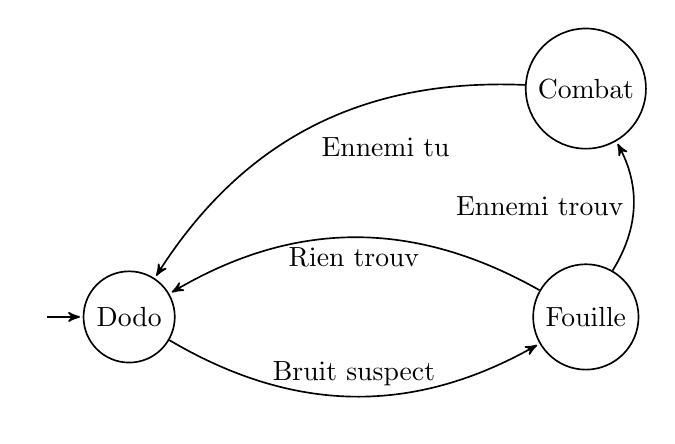
\begin{tikzpicture}[->,>=stealth',shorten >=1pt,auto,node distance=2.9cm,
                    semithick]
  \tikzstyle{every state}=[fill=white,text=black]
  \tikzstyle{place}=[rectangle,draw=black,fill=white, minimum size=7mm]


  \node[initial,state] (A)                    {Dodo};
  \node[] (D) [right of=A] {} ;
  \node[state] (B)      [right of=D]                {Fouille};
  \node[state] (C)      [above of=B]                {Combat};

  \path %(I) edge[loop above]              node {$a,b$} (I)
(A) edge      [bend right]        node {Bruit suspect} (B)
(B) edge      [bend right]        node {Rien trouvé} (A)
(B) edge      [bend right]        node {Ennemi trouvé} (C)
(C) edge      [bend right]        node {Ennemi tué} (A);
\end{tikzpicture}
\caption{Comportement des gardes d'un jeu imaginaire}
\label{garde}
\end{figure}

Ce qu'est censé traduire ce graphe, c'est qu'un garde commence (la $\rightarrow$ sur sa gauche) dans un \textbf{état} qui est le dodo, et que différents événements (un bruit, un ennemi trouvé ou non, ou encore tué) vont le faire changer d'\textbf{état}. Un AFD fonctionne sur un principe similaire\footnote{Les AFD sont en fait des cas particuliers de Machines à états finis, \href{https://www.youtube.com/watch?v=JyF0oyarz4U}{qui sont effectivement employées dans la conception de jeux vidéo}}, mais où les transitions sont déclenchées par la lecture de lettres : un $AFD$, en partant d'un état initial, lit le mot donné en argument lettre par lettre et, à chaque lecture, change d'état en fonction de la lettre. 

\begin{example}
L'automate de la figure \ref{aaauto} contient trois états, appelés $0$, $1$ et $2$. La lecture de tout mot commence en $0$, appelé \textbf{état initial}. Si on lui passe le mot $abbaaba$ en argument, la première lettre ($a$) va nous faire passer de l'état $0$ à $1$. La deuxième lettre ($b$) nous refait passer en $0$. La troisième ($b$) nous y fait rester. Les deux lettres suivantes nous font ensuite passer en $1$ puis en $2$. Les deux dernières lectures nous font rester en $2$ (la virgule est à comprendre comme une disjonction, cad. comme un "ou").
\end{example}



\begin{figure}[!h]
\centering
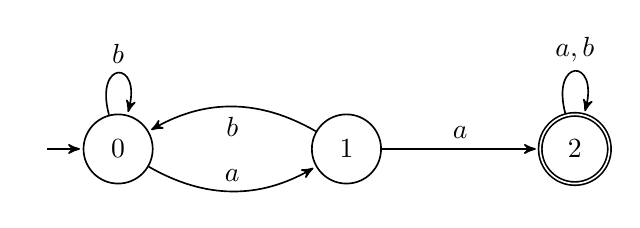
\begin{tikzpicture}[->,>=stealth',shorten >=1pt,auto,node distance=2.9cm,
                    semithick]
  \tikzstyle{every state}=[fill=white,text=black]
  \tikzstyle{place}=[rectangle,draw=black,fill=white, minimum size=7mm]


  \node[initial,state] (A)                    {$0$};
  \node[state] (B)      [right of=A]                {$1$};
  \node[accepting,state] (C)      [right of=B]                {$2$};

  \path %(I) edge[loop above]              node {$a,b$} (I)
(A) edge      [loop above]        node {$b$} (A)
(C) edge      [loop above]        node {$a,b$} (C)
(A) edge      [bend right]        node {$a$} (B)
(B) edge      [bend right]        node {$b$} (A)
(B) edge      []        node {$a$} (C);
\end{tikzpicture}
\caption{Un premier automate}
\label{aaauto}
\end{figure}

Comme dit en introduction, un automate accepte ou rejette tout mot donné. Certains états, notés par une douche couche, sont appelés états finaux (ou terminaux). Un mot est accepté par un automate si et seulement si le parcours de ce mot dans l'automate se termine sur un état final.

\begin{example}
L'automate de la figure \ref{aaauto} accepte le mot $abbaaba$, puisqu'il nous fait passer de l'état initial $0$ à $2$, qui est un état final. Il n'accepte en revanche pas les mots $bbaba$ (état $1$), $babbab$ ou $\epsilon$ (état $0$ tous les deux).
\end{example}

\begin{exercice}
Les mots $abbaba$, $ababbaab$ et $abba$ sont-ils acceptés par l'automate de la figure \ref{aaauto} ?
\end{exercice}

\begin{exercice}
Quel est le \textbf{langage reconnu}, cad. l'ensemble des mots acceptés, par l'automate de la figure \ref{aaauto} ? Donner la réponse en français et sous forme d'expression rationnelle.
\end{exercice}

\paragraph*{Remarque} Un automate ne contient pas toujours une transition pour chaque couple d'état / lettre, auquel cas il est dit \textbf{incomplet}. Si un automate ne contient pas de chemin correspondant à un mot, ce dernier est rejetté.

\begin{example}
L'automate de la figure \ref{incompauto} rejette le mot $aba$, car il n'y a pas de transition partant de l'état $1$ pour la lettre $b$.
\end{example}


\begin{figure}[!h]
\centering
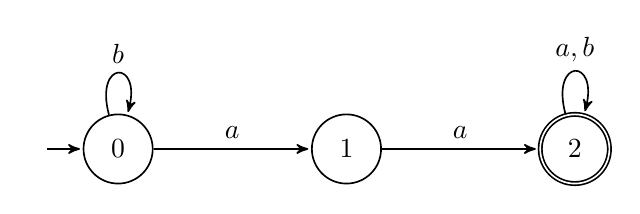
\begin{tikzpicture}[->,>=stealth',shorten >=1pt,auto,node distance=2.9cm,
                    semithick]
  \tikzstyle{every state}=[fill=white,text=black]
  \tikzstyle{place}=[rectangle,draw=black,fill=white, minimum size=7mm]


  \node[initial,state] (A)                    {$0$};
  \node[state] (B)      [right of=A]                {$1$};
  \node[accepting,state] (C)      [right of=B]                {$2$};

  \path %(I) edge[loop above]              node {$a,b$} (I)
(A) edge      [loop above]        node {$b$} (A)
(C) edge      [loop above]        node {$a,b$} (C)
(A) edge      []        node {$a$} (B)
(B) edge      []        node {$a$} (C);
\end{tikzpicture}
\caption{Un automate incomplet}
\label{incompauto}
\end{figure}


\begin{exercice}
Les mots $bbbaababbaaba$, $bbabaab$ et $baaaaaab$ sont-ils acceptés par l'automate de la figure \ref{incompauto} ?
\end{exercice}

\begin{exercice}
Quel est le langage reconnu par l'automate de la figure \ref{incompauto} ? Donner la réponse en français et sous forme d'expression rationnelle.
\end{exercice}


Il nous semble important d'insister sur le point suivant : de la même façon qu'un programme devrait la traduction d'une logique sous-jacente plutôt qu'un bidouaille fait à la va-vite, les états d'un automate ont un sens. Avant d'écrire un automate, il convient donc de réfléchir quelles sont les informations à retenir au cours de la lecture du mot. Si la bonne réponse est trouvée, le reste de l'automate devrait s'écrire seul.

\begin{example}
\label{exemplePI}
On veut écrire un automate reconnaissant le langage $L = \{w \in \Sigma^*~|~|w|_a$ pair et $|w|_b$ impair$\}$, cad. l'ensemble des mots avec un nombre pair de $a$ et impairs de $b$\footnote{On conseillera tout d'abord au lecteur ou à la lectrice de tenter lui/elle-même l'exercice, afin de mesurer la pertinence de l'approche ici présentée}.

Il n'est pas question de compter les $a$ et les $b$ comme on pourrait naïvement l'imaginer, non seulement puisqu'il faut se contenter d'un nombre fini d'états, mais aussi parce que c'est beaucoup plus d'information que nécessaire.
Les seules données qui nous intéressent sont en effet la parité du nombre de $a$ et du nombre de $b$ du mot donné : $a^2b$ comme $a^{26}b^{131}$ sont équivalents dans leur appartenance à $L$.

Le nombre de $a$ et de $b$ étant tous les deux pairs ou impairs, on a 4 possibilités. Nos états s'appeleront $PP$ (nombre de $a$ pair et nombre de $b$ pair), $PI$ ($a$ pair et $b$ impair), $IP$ et $II$. La définition de $L$ nous dit immédiatement que seul $PI$ devrait être terminal. L'état initial devrait être celui qui correspond à $\epsilon$, cad. $PP$.

Les transitions s'écrivent naturellement : en partant de $PP$, la lecture d'un $a$ change la parité du nombre de $a$ mais pas celle du nombre de $b$, et nous emmène donc vers $IP$, tandis que $b$ pointe vers $PI$, et ainsi de suite. S'il y a d'autres lettres dans l'alphabet, elles devraient faire des boucles, puisqu'elles ne changent rien aux parités qui nous intéressent.

Au final, on obtient l'automate suivant : 


\centering
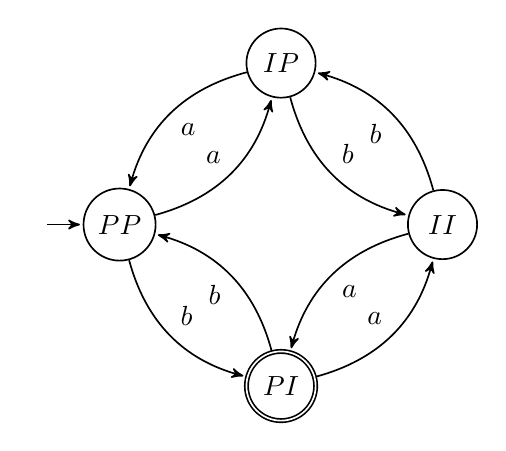
\begin{tikzpicture}[->,>=stealth',shorten >=1pt,auto,node distance=2.9cm,
                    semithick]
  \tikzstyle{every state}=[fill=white,text=black]
  \tikzstyle{place}=[rectangle,draw=black,fill=white, minimum size=7mm]


  \node[initial,state] (PP)                    {$PP$};
  \node[state] (IP)      [above right of=PP]                {$IP$};  \node[state] (II)      [below right of=IP]                {$II$};
  \node[accepting,state] (PI)      [below right of=PP]                {$PI$};

  \path %(I) edge[loop above]              node {$a,b$} (I)
(PP) edge      [bend right]        node {$a$} (IP)
(PP) edge      [bend right]        node {$b$} (PI)
(PI) edge      [bend right]        node {$a$} (II)
(PI) edge      [bend right]        node {$b$} (PP)
(IP) edge      [bend right]        node {$a$} (PP)
(IP) edge      [bend right]        node {$b$} (II)
(II) edge      [bend right]        node {$a$} (PI)
(II) edge      [bend right]        node {$b$} (IP);
\end{tikzpicture}
\end{example}

\begin{exercice} (**) En reprenant l'exemple \ref{exemplePI}, montrer que $\forall w, w \in L \leftrightarrow$ l'automate accepte $w$. Vous pouvez procéder par induction sur $w$, en utilisant un objectif un peu plus précis que celui fourni.
\end{exercice}

Dans la série d'exercices qui suit, on utilisera comme alphabet $\Sigma = \{a,b\}$.

\begin{exercice}
Donner un automate qui reconnaît le langage $\{w \in \Sigma^*~|~|w| \geq 3\}$. 
\end{exercice}

\begin{exercice}
Donner un automate pour les mots qui commencent par $a$.
\end{exercice}

\begin{exercice}
Donner un automate pour les mots qui finissent par $b$.
\end{exercice}

\begin{exercice}
Donner un automate pour les mots qui commencent par $a$ finissent par $b$.
\end{exercice}


\begin{exercice}
Donner un automate pour les mots de longueur paire.
\end{exercice}

\begin{exercice}
Donner un autuomate pour les mots de longueur impaire qui contiennent au moins 4 lettres.
\end{exercice}

\begin{exercice}
Donner un automate pour les mots de longueur impaire, qui contiennent au moins 4 lettres, commencent par $a$ et finissent par $b$.
\end{exercice}

\subsection{Formalisation et implémentation}

Un automate fini déterministe est un $5-uplet$ (cad. un "paquet" qui contient 5 éléments ordonnés)

\[
%A =  
\big \langle Q,\Sigma,q_0,F,\delta \big \rangle
\]

avec

\begin{itemize}
\item[] $Q$ ensemble fini d'états
\item[] $\Sigma$ l'alphabet
\item[] $q_0$ l'état initial
\item[] $F \subseteq Q$, les états terminaux
\item[] $\delta$ fonction partielle\footnote{Une fonction partielle est une fonction qui n'attribue pas forcément une image à tout argument. Dans le cas d'un automate complet, la fonction de transition est donc une fonction totale.} de $Q \times \Sigma$ dans $Q$ 
\end{itemize}

La fonction $\delta$ est alors \textit{liftée} aux mots\footnote{On dit qu'une fonction est \textit{liftée} lorsqu'on "soulève" le type d'un ou plusieurs de ses arguments, pour qu'elle s'applique par exemple à des listes ou des ensembles. Typiquement, si on a une fonction $f$ de type $\mathbb{N} \rightarrow \mathbb{N}$, alors sa version \textit{liftée} aux listes, étant donnée une liste $[a_1,...,a_n]$, renverra $[f(a_1),...,f(a_n)]$.} pour obtenir la fonction $\delta^* : (Q \times \Sigma^*) \rightarrow$ définie de la façon suivante :

\begin{itemize}
\item $\delta^*(q,\epsilon) = q$
\item $\delta^*(q,a.w) = \delta^*(\delta(q,a),w)$ ($a$ est une lettre et $w$ un mot, éventuellement vide)
\end{itemize}

Plus prosaïquement, la fonction $\delta^*$ applique $\delta$ sur $w$, lettre par lettre, de la gauche vers la droite. Dans ce cadre, on dit qu'un mot $w$ est \textbf{reconnu} (ou accepté) par l'automate ssi. $\delta^*(q_0,w) \in F$. Dit encore autrement, un mot est accepté ssi en partant de l'état initial de l'automate et en suivant les transitions correspondant aux lettres successives du mot on finit dans un état terminal. 

La définition de $\delta^*$ donne quasiment directement une implémentation de la reconnaissance via automate fini déterministe :
\begin{figure}[!ht]
\begin{python}
state = q_0
for c in w:
    state = delta(state,c)
return (state in F)
\end{python}
\caption{Reconnaissance par un AFD}
\label{afdrec}
\end{figure}

\begin{example}
L'automate de la figure \ref{aaauto} se formalise de la façon suivante :

\begin{itemize}
\item $Q = \{0,1,2\}$
\item $\Sigma = \{a,b\}$
\item $q_0 = 0$
\item $F = \{2\}$
\item $\delta(0,a) = 1; \delta(0,b) = 0; \delta(1,a) = 2; \delta(1,b) = 0; \delta(2,a) = 2; \delta(2,b) = 2$
\end{itemize}

On peut vérifier qu'il accepte bien le mot $abbaaba$ (lecture comme une BD) :

\begin{tabular}{lllll}
$\delta^*(0,abbaaba)$ &$=$& $\delta^*(\delta(0,a),bbaaba)$& $=$&$\delta^*(1,bbaaba)$ \\
&$=$& $\delta^*(\delta(1,b),baaba)$ &$=$& $\delta^*(0,baaba) $\\
&$=$& $\delta^*(\delta(0,b),aaba)$ &$=$& $\delta^*(0,aaba) $\\
&$=$& $\delta^*(\delta(0,a),aba)$ &$=$& $\delta^*(1,aba) $\\
&$=$& $\delta^*(\delta(1,a),ba)$ &$=$& $\delta^*(2,ba) $\\
&$=$& $\delta^*(\delta(2,b),a)$ &$=$& $\delta^*(2,a) $\\
&$=$& $\delta^*(\delta(2,a),\epsilon)$ &$=$& $\delta^*(2,\epsilon) $\\
&&&$=$&$2 \in F$
\end{tabular}


\end{example}

\begin{exercice}
Donner la formalisation de l'automate de l'exemple \ref{exemplePI} et vérifier qu'il accepte le mot $aababba$. 
\end{exercice}

On a introduit en \ref{reappart} l'expression rationnelle $e = ((\Sigma^*baaba^+)^*baa(abba)^+ba(bb)^*a)^*$, qu'on était censé traduire en programme via les automates finis. Or, la traduction en AFD n'est à priori pas si évidente que ça (on conseille à nouveau d'essayer pour se rendre compte de la difficulté), du fait du haut niveau de non-déterminisme dans la \textit{regex}. On va donc avoir besoin d'un modèle un peu plus permissif.

\section{Automates finis non-déterministes}
\label{NDFA}

Les automates finis qu'on a vus jusqu'ici sont déterministes, en ce qu'un automate admet au maximum une seule transition par lettre, et donc que tout mot n'a lui-même pas plus d'un chemin. On va ici voir une nouvelle classe d'automates, les automates finis non-déterministes (AFND, ou \textit{NDFA} pour \textit{non-deterministic finite automaton/a}), qui vont justement nous libérer de cette contrainte.

\subsection{Principe général}

Le non-déterminisme se manifeste de deux façons. On a d'abord les $\epsilon$-transitions, qui seront étudiées à part dans le cadre d'un DM. Ici, on se concentrera sur la possibilité d'avoir plusieurs transitions pour le même couple état $\times$ lettre, ainsi que plusieurs états initiaux.

On peut donc maintenant avoir dans un automate plusieurs chemins pour un même mot, chemins qui vont chacun mener ou non à un état terminal. On accepte tout mot qui mène à un état terminal via au moins un chemin.

\begin{example}
Le langage des mots qui contiennent le facteur $aba$, dénoté par la \textit{regex} $\Sigma^*aba\Sigma^*$, est reconnu par l'automate suivant :

\begin{figure}[!ht]
\centering
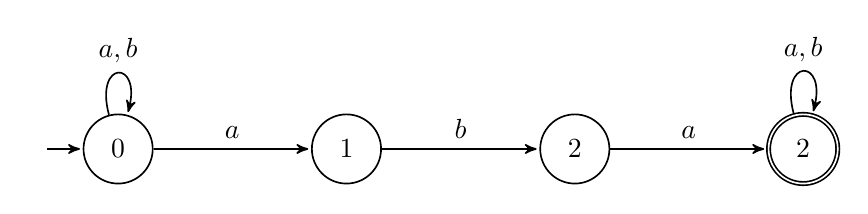
\begin{tikzpicture}[->,>=stealth',shorten >=1pt,auto,node distance=2.9cm,
                    semithick]
  \tikzstyle{every state}=[fill=white,text=black]
  \tikzstyle{place}=[rectangle,draw=black,fill=white, minimum size=7mm]


  \node[initial,state] (0)                    {$0$};
  \node[state] (1)      [right of=0]                {$1$};  
  \node[state] (2)      [right of=1]                {$2$};
  \node[accepting,state] (3)      [right of=2]                {$2$};

  \path %(I) edge[loop above]              node {$a,b$} (I)
(0) edge      [loop above]        node {$a,b$} (0)
(0) edge      []        node {$a$} (1)
(1) edge      []        node {$b$} (2)
(2) edge      []        node {$a$} (3)
(3) edge      [loop above]        node {$a,b$} (3);
\end{tikzpicture}
\end{figure}

Si on regarde par exemple le mot $aabab$, il dispose de 3 parcours dans l'automate : 

\begin{itemize}
\item $0 \xrightarrow{a} 0 \xrightarrow{a} 0 \xrightarrow{b} 0 \xrightarrow{a} 0 \xrightarrow{b} 0$
\item $0 \xrightarrow{a} 0 \xrightarrow{a} 0 \xrightarrow{b} 0 \xrightarrow{a} 1 \xrightarrow{b} 2$
\item $0 \xrightarrow{a} 0 \xrightarrow{a} 1 \xrightarrow{b} 2 \xrightarrow{a} 3 \xrightarrow{b} 3$
\end{itemize}

On peut aussi passer dans l'état $1$ avec le premier $a$, mais il sera alors impossible de lire l'entiéreté du mot (le deuxième $a$ n'aura pas de transition).

Des trois chemins possibles, un seul mène à un état terminal. C'est néanmoins suffisant pour que le mot soit accepté. A l'inverse, le mot $abbaabbaaabba$, bien que pouvant faire de très nombreux chemins dans l'automate, n'est pas accepté car aucun ne finit en $3$
\end{example}

Un tel automate a l'avantage de reconnaître très clairement le langage $\Sigma^*aba\Sigma^*$. On peut par exemple le comparer à sa version déterministe qui, malgré la simplicité du langage, perd déjà pas mal en lisibilité :

\begin{figure}[!ht]
\centering
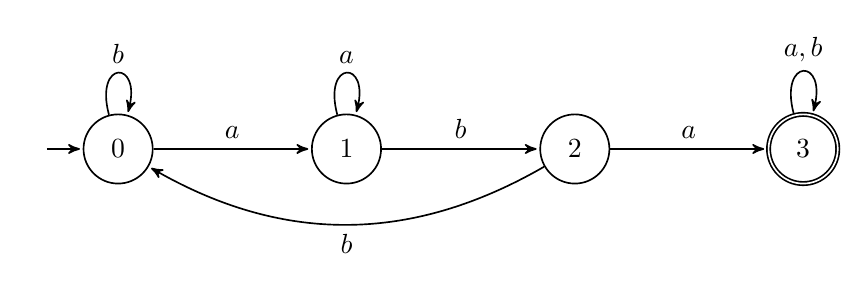
\begin{tikzpicture}[->,>=stealth',shorten >=1pt,auto,node distance=2.9cm,
                    semithick]
  \tikzstyle{every state}=[fill=white,text=black]
  \tikzstyle{place}=[rectangle,draw=black,fill=white, minimum size=7mm]


  \node[initial,state] (0)                    {$0$};
  \node[state] (1)      [right of=0]                {$1$};  
  \node[state] (2)      [right of=1]                {$2$};
  \node[accepting,state] (3)      [right of=2]                {$3$};

  \path %(I) edge[loop above]              node {$a,b$} (I)
(0) edge      [loop above]        node {$b$} (0)
(0) edge      []        node {$a$} (1)
(1) edge      [loop above]        node {$a$} (1)
(1) edge      []        node {$b$} (2)
(2) edge      []        node {$a$} (3)
(2) edge      [bend left]        node {$b$} (0)
(3) edge      [loop above]        node {$a,b$} (3);
\end{tikzpicture}
\end{figure}

La grande différence entre les deux automates est que le premier utilise le non-déterminisme pour être une transcription directe de la \textit{regex}, là où le deuxième se bat avec le déterminisme pour reconnaître le langage de façon presque "accidentelle". En un sens, on est passé du domaine de la \textbf{spécification} à l'\textbf{implémentation}. La mauvaise nouvelle, c'est que les automates non-déterministes sont plus compliqués à mettre en pratique, du fait - ô surprise - du non-déterminisme, qui impose de tester énormément de chemins. La bonne nouvelle, c'est que, comme on va le voir en \ref{det}, on peut traduire automatiquement les automates non-déterministes en automates déterministes équivalents\footnote{Pour se rendre compte du miracle que c'est, on peut comparer aux langages de programmation classiques. Ce n'est pas parce qu'on a spécifié formellement, par exemple, le tri d'une liste (ce qui est déjà surprenamment non-trivial) qu'on peut automatiquement obtenir un programme réalisant cette tâche. Même une fois qu'on a codé un tel programme, selon l'algorithme chopisi, il n'est pas forcément aisé de se convaincre qu'il est correct, et encore moins de le prouver formellement. Il est donc assez \textit{cool} que tout ce passage de la spécification (la \textit{regex}) à une représentation intermédiaire (l'automate non-déterministe) à l'implémentation (le déterministe) soit automatique et sûre.}, avec bien sûr un certain coût. Mais avant de plonger dans ces histoires, on va voir encore quelques exemples d'AFND, et en étudier la formalisation.

\begin{example}
On veut reconnaître le langage des mots qui contiennent le facteur $aba$ ou (inclusif) $bab$. On peut exploiter la possibilité d'avoir plusieurs états initiaux, et tout simplement produire l'automate suivant :

\begin{figure}[!ht]
\centering
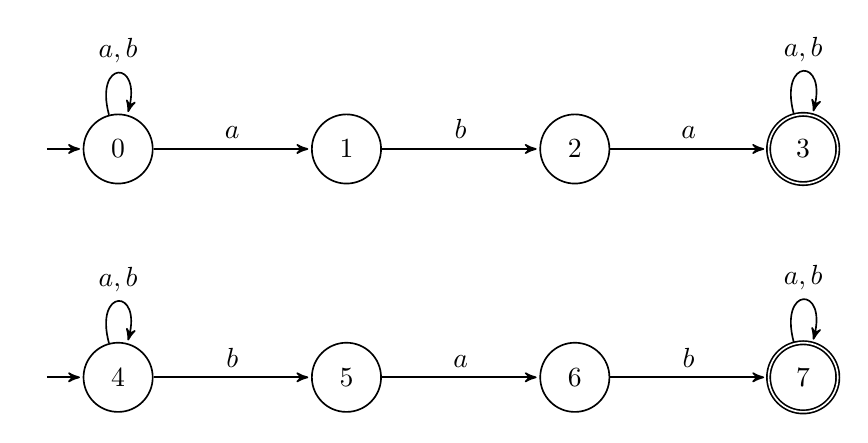
\begin{tikzpicture}[->,>=stealth',shorten >=1pt,auto,node distance=2.9cm,
                    semithick]
  \tikzstyle{every state}=[fill=white,text=black]
  \tikzstyle{place}=[rectangle,draw=black,fill=white, minimum size=7mm]


  \node[initial,state] (0)                    {$0$};
  \node[state] (1)      [right of=0]                {$1$};  
  \node[state] (2)      [right of=1]                {$2$};
  \node[accepting,state] (3)      [right of=2]                {$3$};

  \node[initial,state] (4)  [below of=0]            {$4$};
  \node[state] (5)      [right of=4]                {$5$};  
  \node[state] (6)      [right of=5]                {$6$};
  \node[accepting,state] (7)      [right of=6]                {$7$};

  \path %(I) edge[loop above]              node {$a,b$} (I)
(0) edge      [loop above]        node {$a,b$} (0)
(0) edge      []        node {$a$} (1)
(1) edge      []        node {$b$} (2)
(2) edge      []        node {$a$} (3)
(3) edge      [loop above]        node {$a,b$} (3)
(4) edge      [loop above]        node {$a,b$} (4)
(4) edge      []        node {$b$} (5)
(5) edge      []        node {$a$} (6)
(6) edge      []        node {$b$} (7)
(7) edge      [loop above]        node {$a,b$} (7);

\end{tikzpicture}
\end{figure}

On notera bien sûr la symétrie entre l'automate ci-dessus, et la regex $\Sigma^*aba\Sigma^* + \Sigma^*bab\Sigma^*$.

On peut aussi tenter d'être un poil plus malin, se rendre compte que les états $0$ et $4$ ont le même \textbf{rôle}, que les états $3$ et $7$ aussi, et donc qu'on peut réduire le nombre d'états en les fusionnant :


\begin{figure}[!ht]
\centering
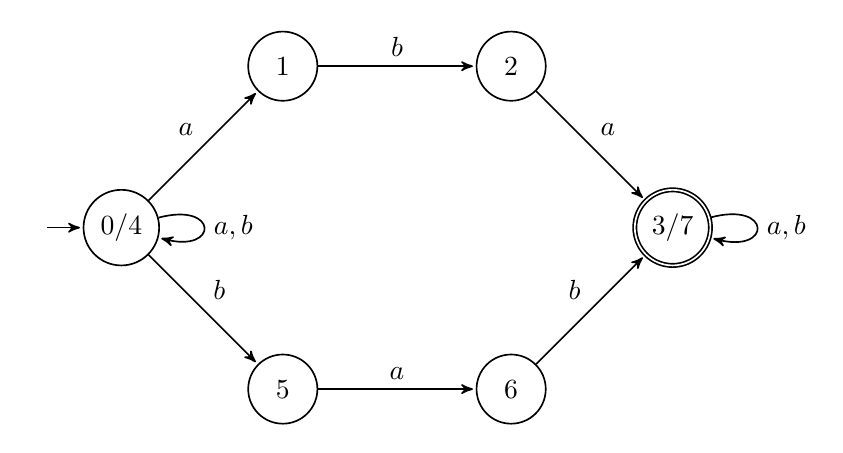
\begin{tikzpicture}[->,>=stealth',shorten >=1pt,auto,node distance=2.9cm,
                    semithick]
  \tikzstyle{every state}=[fill=white,text=black]
  \tikzstyle{place}=[rectangle,draw=black,fill=white, minimum size=7mm]


  \node[initial,state] (0)                    {$0/4$};
  \node[state] (1)      [above right of=0]                {$1$};  
  \node[state] (2)      [right of=1]                {$2$};
  \node[state] (3)      [below right of=0]                {$5$};  
  \node[state] (4)      [right of=3]                {$6$};
  \node[accepting,state] (5)      [below right of=2]                {$3/7$};

  \path %(I) edge[loop above]              node {$a,b$} (I)
(0) edge      [loop right]        node {$a,b$} (0)
(0) edge      []        node {$a$} (1)
(0) edge      []        node {$b$} (3)
(1) edge      []        node {$b$} (2)
(3) edge      []        node {$a$} (4)
(2) edge      []        node {$a$} (5)
(4) edge      []        node {$b$} (5)
(5) edge      [loop right]        node {$a,b$} (5);

\end{tikzpicture}
\end{figure}
\newpage
Cette notion d'états équivalents et fusionnables sera formalisée en \ref{minim}. On remarquera (à nouveau) la symétrie entre cet automate et la regex $\Sigma^*(aba+bab)\Sigma^*$.

\end{example}

\begin{exercice}
Donner une \textit{regex} et un automate fini pour le langage $L = \{w ~|~ aba$ est un sous-mot de $w\}$.
\end{exercice}


\begin{exercice}
Donner une \textit{regex} et un automate fini pour le langage des mots qui commencent par $ab$ et finissent par $ba$.
\end{exercice}

\subsection{Formalisation et implémentation}

Les automates non-déterministes sont une généralisation\footnote{En effet, un AFD peut-être vu comme un AFND qui se trouve être ... déterministe. Rien dans la définition d'un AFND n'impose que le non-déterminisme permis par le changement de type de $\delta$ soit exploité, et on peut donc très bien avoir $|\delta(q,c)| \leq 1~\forall q \in Q$ et $\forall c \in \Sigma$.} des automates déterministes, où
 
\begin{itemize}
\item L'état initial $q_0$ est remplacé par un ensemble d'états initiaux $I \subseteq Q$
\item La fonction de transition $\delta$ change de type, en passant de $(Q \times \Sigma) \rightarrow Q$ à $(Q \times \Sigma) \rightarrow P(Q)$\footnote{Pour rappel, $P(Q)$ est l'ensemble des sous-parties de $Q$, cad. l'ensemble des ensembles d'états, cf \ref{powerset}.}. Dit autrement, étant donnés un état $q \in Q$ et une lettre $c \in \Sigma$, on a (potentiellement) \textit{accès} à un ensemble d'états plutôt qu'à un seul.
\end{itemize}


Puisqu'on a changé le type $\delta$, on doit également changer son \textit{lift} $\delta^*$, qui renvoie maintenant un ensemble d'états et est donc de type $(Q \times \Sigma^*) \rightarrow P(Q)$ :
 
\begin{itemize}
\item $\delta^*(q,\epsilon) = \{q\}$
\item $\delta^*(q,a.w) = \bigcup_{q' \in \delta(q,a)} \delta^*(q',w)$
\end{itemize}


Pour ce qui est de la mise en application de $\delta^*$, on est cette fois face à un parcours d'arbres (l'ensemble des chemins) plutôt que d'une liste, comme dans la version déterministe. On adapte donc l'annexe \ref{itersif} :

\begin{figure}[!ht]
\begin{python}
# fonction ndfa_acc(auto,w)
# renvoie true ssi. l automate auto accepte le mot w
todo = stack()
// On va empiler des couples etat x mot qu il faut tester
// On commence par se noter tous les etats initiaux
for i in initial(auto):
    todo.add(i,w)
while (todo pas vide):
    (q,mot) = todo.pop()
    // Si on a fini de lire le mot et qu on est
    // arrive sur un etat final, on accepte
    // Si l etat n est pas final, on ne renvoie
    // pas false, car il peut rester des chemins
    // qu il faut tester
    if mot is empty et q in F:
        return true 
    elif mot is a.reste:
        // On continue la lecture du mot avec 
        // chaque etat qu on peut atteindre
        // avec la premiere lettre
        next_states = delta(q,a)
        for suivant in next_states:
            todo.add(suivant,reste)
// Si on n a au final rien trouve, on dit non
return false
\end{python}
\caption{Reconnaissance par un AFND - version iterative}
%\label{treeit}
\end{figure}

\begin{figure}[!ht]
\begin{python}
# fonction ndfa_acc_bis(auto,w,q)
# renvoie true ssi. l automate auto accepte le mot w en partant de l etat q
if w is empty:
    return q in F
elif w is a.reste:
    for suivant in delta(q,a):
        if ndfa_acc_bis(auto,reste,suivant):
            return true
    return false


# fonction ndfa_acc(auto,w)
# renvoie true ssi. l automate auto accepte le mot w
for i in initial(auto):
    if ndfa_acc_bis(auto,w,i):
        return true
return false
\end{python}
\caption{Reconnaissance par un AFND - version récursive}
%\label{treerec}
\end{figure}
\newpage

\section{Transformation d'automates}
\label{transauto}

%La formalisation très limitée et simple des automates en fait des programmes particulièrement simple à manipuler, comme l'illustrent les algorithmes de transformation d'automates présentés ici.

\subsection{Complétion}

\subsection{Déterminisation}
\label{det}

\subsection{Minimisation}
\label{minim}

\section{Propriétés de clôture}
\label{cloture}
\subsection{Union}

\subsection{Intersection}

\subsection{Concaténation}

\subsection{Itération}



\chapter{Grammaires formelles et hiérarchie de Chomsky}
\label{grammaires}


\section{Principe général}

Une \textbf{grammaire formelle} est une série de \textbf{règles} permettant de générer des mots. Ces règles utilisent des \textbf{symboles} dits \textbf{terminaux} (les lettres "normales", par convention en minuscules), et d'autres dits \textbf{non-terminaux} (normalement dénotés par des lettres majuscules). Un de ces symboles non-terminaux, appelé \textbf{axiome}, indique le début de toute génération de mot. On présente d'abord le fonctionnement des grammaires et les concepts de base à l'aide de quelques exemples. 

\begin{example}
On présente la grammaire dénotée par ces deux règles :

\[
\begin{cases}
S \rightarrow \epsilon \\
S \rightarrow abS 
\end{cases}
\]

Cette grammaire contient un seul symbole non-terminal, S. Il s'agit donc automatiquement de l'axiome. Le symbole S peut se transformer en $\epsilon$ (première règle) ou en $abS$ (deuxième règle). Cette grammaire génère l'ensemble des mots composés uniquement de symboles terminaux ($a$ et $b$) qu'on peut obtenir en partant de l'axiome S et en appliquant autant de fois qu'on veut les règles données. Dans ce qui suit, on écrira $\rightarrow_1$ pour une application de la première règle et $\rightarrow_2$ pour la seconde.

On peut par exemple obtenir le mot $ab$ de la façon suivante :

\[
S \rightarrow_2 abS \rightarrow_1 ab
\]

Dans cette suite de transformation, appelée \textbf{dérivation}, on remplace d'abord l'axiome par $abS$ à l'aide de la deuxième règle. Puisque $abS$ contient le facteur $S$, on peut utiliser \textit{localement} la deuxième règle pour faire disparaître ce S. Dans ce cas, ce qu'il y avait autour du S, le \textbf{contexte}, reste inchangé.

On peut également obtenir le mot $abab$ :

\[
S \rightarrow_2 \textcolor{blue}{ab}S \rightarrow_2 \textcolor{blue}{ab}\textcolor{red}{ab}S \rightarrow_1 \textcolor{blue}{ab}\textcolor{red}{ab}
\]

ou ababab :


\[
S \rightarrow_2 \textcolor{blue}{ab}S \rightarrow_2 \textcolor{blue}{ab}\textcolor{red}{ab}S \rightarrow_2 \textcolor{blue}{ab}\textcolor{red}{ab}\textcolor{green}{ab}S \rightarrow_1  \textcolor{blue}{ab}\textcolor{red}{ab}\textcolor{green}{ab}
\]

Il n'est pas obligatoire d'utiliser toutes les règles d'une grammaire. On peut donc générer le mot vide :

\[
S \rightarrow_1 \epsilon
\]

On se rend compte assez vite que la grammaire \textbf{engendre} le langage $(ab)^*$.

\end{example}


\begin{example}
\label{LRgram}
Un symbole non-terminal peut générer d'autres symboles non-terminaux, et même plusieurs en même temps. De plus, un non-terminal peut générer un autre mot que juste $\epsilon$. Ces deux points sont illustrés par la grammaire suivante :

\[
\begin{cases}
S \rightarrow LaaR \\
L \rightarrow Lb \\
L \rightarrow ab \\
R \rightarrow bR \\
R \rightarrow ba
\end{cases}
\]

Quelques exemples de dérivations dans cette grammaire :

\[
 S \rightarrow_1 LaaR \rightarrow_2 LbaaR \rightarrow_2 LbbaaR \rightarrow_4 LbbaabR \rightarrow_3 abbbaabR \rightarrow_5 abbbaabba
\]

\[
 S \rightarrow_1 LaaR \rightarrow_3 abaaR \rightarrow_5 abaaba
 \]
 
 On note $\rightarrow_i^j$ $j$ utilisations de la règle numéro $i$, comme dans la dérivation suivante :
 
 \[
 S \rightarrow_1 LaaR \rightarrow_2^5 LbbbbbaaR \rightarrow_3 abbbbbbaaR \rightarrow_4^3 abbbbbbaabbbR \rightarrow_5 abbbbbbaabbbba
 \]

\end{example}

\begin{exercice}
Quel est le langage engendré par la grammaire de l'exemple \ref{LRgram} ?
\end{exercice}

\begin{exercice}
\label{grammab}
Quel est le langage reconnu par la grammaire suivante ?

\[
\begin{cases}
S \rightarrow A \\
S \rightarrow B \\
A \rightarrow aA \\
A \rightarrow \epsilon \\
B \rightarrow bB \\
B \rightarrow \epsilon
\end{cases}
\]

\end{exercice}

\begin{exercice}
\label{grammsigma}
Quel est le langage reconnu par la grammaire suivante ?

\[
\begin{cases}
S \rightarrow aS \\
S \rightarrow bS \\
S \rightarrow \epsilon 
\end{cases}
\]

\end{exercice}

\begin{exercice}
Donner l'ensemble des mots qui admettent deux dérivations (ie. peuvent être construits de plusieurs façons différentes) dans la grammaire de l'exercice \ref{grammab}. Même question pour celle de l'exercice \ref{grammsigma}.
\end{exercice}

\begin{example}
\label{ggramabcn}
On a jusqu'ici seulement vu des exemples de grammaires avec un seul non-terminal à gauche des flèches de réécriture. Il est cependant possible de préciser le contexte dans lequel les réécritures doivent se faire, comme dans la grammaire suivante :

\[
\begin{cases}
S \rightarrow SABC \\
S \rightarrow \epsilon \\
AB \rightarrow BA \\
BA \rightarrow AB \\
AC \rightarrow CA \\
CA \rightarrow AC \\
BC \rightarrow CB \\
CB \rightarrow BC \\
A \rightarrow a \\
B \rightarrow b \\
C \rightarrow c
\end{cases}
\]

Toute dérivation dans cette grammaire fonctionne de la façon suivante : on commence par utiliser la première règle $n$ fois pour produire $S(ABC)^n$. Ensuite, on utilise la deuxième règle pour faire disparaître S et se retrouver avec $(ABC)^n$. Les règles 3 à 8 permettent ensuite de mélanger les symboles non-terminaux comme on l'entend. Une fois qu'ils ont été disposés de la façon voulue, on les transforme en $a$, $b$ et $c$ avec les règles 9, 10 et 11.

Le langage engendré par cette grammaire est donc celui des mots contenant autant de $a$ que de $b$ et de $c$.
\end{example}

\paragraph{Remarque} Dans l'exemple ci-dessus, on découpe toute dérivation en 4 étapes : utilisation de la première règle, puis de la seconde, puis des 3 à 8, et enfin des 9 à 11. Cette présentation nous semble améliorer la compréhension de l'exemple et du langage engendré, mais techniquement, rien n'empêche de mélanger les étapes, comme dans la dérivation suivante :

 \[
 S \rightarrow_1 SABC \rightarrow_9 SaBC \rightarrow_7 SaCB \rightarrow_{11} SaCb \rightarrow_1 SABCaCb \rightarrow_2 ABCaCB \rightarrow_{9,10,11}^5 abcacb 
 \]

 Où $\rightarrow_{9,10,11}^5$ indique 5 utilisations de règles parmi 9, 10 et 11.
 
 \section{Formalisation}
 
 Maintenant qu'on a un peu joué avec les grammaires formelles, on peut regarder comment elles se formalisent. Techniquement donc, une grammaire formelle est un quadruplet $\big \langle\Sigma, V, S, R \big \rangle$, où
 
 \begin{itemize}
 \item $\Sigma$ est l'ensemble des \textbf{symboles terminaux}
 \item $V$ est l'ensemble des \textbf{symboles non-terminaux}
 \item $S \in V$ est l'\textbf{axiome}
 \item $R$ est l'ensemble des \textbf{règles de production}, ou règles de réécriture. Ces dernières forment un sous-ensemble de $(\Sigma \cup V)^*V(\Sigma \cup V)^* \times (\Sigma \cup V)^*$, cad. qu'elles doivent toujours avoir au moins un non-terminal à gauche. 
 \end{itemize}
 
 
 
\begin{example}
La grammaire de l'exemple \ref{LRgram} s'écrit 

\[
\big \langle \{a,b\},\{S,L,R\},S, \begin{cases}
S \rightarrow LaaR \\
L \rightarrow Lb \\
L \rightarrow ab \\
R \rightarrow bR \\
R \rightarrow ba
\end{cases}
 \big \rangle
\]


\begin{definition}{Réécriture / dérivation immédiate}{}
Soient $p$, $s$ et $g$ des mots sur l'alphabet $(\Sigma \cup V)$, et $f \in (\Sigma \cup V)^*V(\Sigma \cup V)^*$. Si la règle $r$ est de la forme $f \rightarrow g$, alors le mot $pfs$ se \textbf{réécrit} (ou dérive) \textbf{immédiatement} en $pgs$ via la règle $r$, ce qu'on note 

\[
pfs \rightarrow_r pgs
\]

Plus généralement, étant donnée une grammaire $G$, on dit qu'elle réécrit (ou dérive) immédiatement un mot $u$ en $v$ ssi. il existe une règle $r$ dans la grammaire telle que $u$ se réécrit immédiatement en $v$ via la règle $r$. On écrit ceci 

\[
pfs \rightarrow_G pgs
\]
\end{definition}

\paragraph{Remarque} $u \rightarrow_r v$ est parfois noté $u \xrightarrow{r} v$. De plus, quand il n'y a pas d'ambiguïté sur la grammaire étudiée, on note $u \rightarrow v$ plutôt que $u \rightarrow_G v$.


\end{example}


\begin{definition}{Réécriture / dérivation}{}
Soient une grammaire $G$ et deux mots $u$ et $v$. On dit que $u$ se \textbf{réécrit} (ou dérive) en $v$ avec $G$ ssi. il existe une série (potentiellement nulle) de réécritures immédiates menant de $u$ à $v$ dans $G$. On le note 

\[
u \rightarrow_G^* v
\]

ou $u \rightarrow^* v$ s'il n'y a pas d'ambiguïté sur la grammaire étudiée.

\end{definition}
 
\begin{example}
Dans l'exemple \ref{ggramabcn}, on a 

\[
S \rightarrow^* SABCaCb \rightarrow^* abcacb
\]

et donc 

\[
S \rightarrow^* abcacb
\]
\end{example}
 
%\begin{definition}{Proto-mot}{}
%Un \textbf{proto-mot} est un mot contenant 
%\end{definition}
% proto-mot, dérivations équivalentes, gauche
% defs utiles dans la suite ?

\begin{definition}{Langage engendré}{}
Le langage engendré par le mot $f$ dans une grammaire $G$, noté $L_G(f)$, est l'ensemble des mots de $\Sigma^*$ (formés uniquement de symboles terminaux) en lesquelles on peut réécrire l'axiome de $f$ en suivant les règles de $G$. Plus formellement,

\[
L_G(f) = \{u \in \Sigma^* ~|~f \rightarrow_G^* u\}
\]

Le langage engendré par une grammaire est le langage engendré par l'axiome dans cette grammaire. Soit une grammaire $G$ d'axiome $S$, son langage engendré, noté $L_G$, est $L_G(S)$.
\end{definition}

\begin{example}
Soit $G$ la grammaire de l'exemple \ref{ggramabcn}. 

\[
L_G = \{w \in \Sigma^* ~|~|w|_a = |w|_b = |w|_c \}
\]
\end{example}

%
\chapter{Notion de calculabilité}

%Pour une version plus détaillée de cette section, voir \cite{dowek}. 
Pour une version plus détaillée, voir \href{https://www.college-de-france.fr/site/xavier-leroy/inaugural-lecture-2018-11-15-18h00.htm}{la leçon inaugurale de Xavier Leroy au Collège de France}.

\section{Différents modèles de calcul}

L'informatique a vocation à automatiser les calculs afin de les faire réaliser par une machine plutôt que par des Humains. Avant d'automatiser les calculs, il s'agit donc de définir formellement de quoi on parle.

D'un point de vue programmation, 2 principaux modèles co-existent : les \textbf{machines de Turing} et le \textbf{$\lambda$-calcul}. Ces langages ne sont pas utilisables en pratique (\href{http://www.ens-lyon.fr/actualite/lecole/la-machine-de-turing-en-legos}{encore que}), mais posent les fondamentaux de ce qu'est un langage de programmation.

\paragraph{Machines de Turing} Les machines de Turing disposent d'une notion d'état, et d'une mémoire infinie modifiable. La notion d'état sera discutée en longueur dans la section \ref{automates}, mais correspond en gros à une mémoire spéciale, propre à chaque programme, qui peut être modifiée et consultée facilement, notamment pour s'orienter dans le \textit{flow} du programme\footnote{Pensez à une variable booleene "premierefois" que vous avez sans doute déjà utilisée dans un \texttt{if} pour accéder ou non à un cas particulier}. Ces traits rapprochement fortement les machines de Turing de la programmation impérative (C, langage machine, le coeur de Python etc). Les machines de Turing sont dues à \textbf{Alan Turing}.

\paragraph{$\lambda$-calcul} A la différence des machines de Turing, qui ont une approche quasiment mécanique (pour ne pas dire "bidouille") de l'exécution d'un programme, le $\lambda$-calcul est profondément mathématique. Tout n'y est que fonction, au point que ces dernières sont des objets comme les autres, notamment passables en arguments. On citera l'exemple classique d'une fonction qui reçoit une fonction de tri et une liste, et renvoie la liste triée selon la fonction fournie. Le $\lambda$-calcul est la base de la programmation fonctionnelle. Il a été crée par \textbf{Alonzo Church}.

\paragraph{Remarque} Les types en programmation impérative n'ont souvent qu'une valeur de garde-fou contre des opérations totalement absurdes, alors qu'ils ont une fonction beaucoup plus structurante (certaine.s diraient "contraignante") en programmation fonctionnelle. L'utilisation de fonctions comme arguments oblige par exemple à repenser les types et aller plus loin que les classiques \verb!bool!, \verb!int! et cie. On renverra encore une fois à la présentation de Xavier Leroy citée en introduction pour une meilleur vision d'ensemble.

Ces deux modèles ne forment pas l'alpha et l'omega de la calculabilité, qui contient de nombreux modèles plus ou moins exotiques, comme les fonctions $\mu$-récursives ou les automates cellulaires (voir à ce sujet \href{https://www.youtube.com/watch?v=S-W0NX97DB0}{la vidéo de la chaîne ScienceEtonnante}).

\paragraph{Thèse de Church (ou thèse de Church-Turing)} Church et Turing ont montré, dans les années 30, que les machines de Turing et le $\lambda$-calcul sont équivalents, dans le sens où toute fonction exprimable dans un modèle le sera dans l'autre. On dit que les modèles ont la même \textbf{expressivité}. Attention cependant, certaines fonctions très simples en $\lambda$-calcul seront un enfer à coder en machine de Turing, et inversement\footnote{Penser à la différence entre compétence et performance.}. Mais il reste remarquable que deux modèles fonctionnant de façons si orthogonales aient, au fond, la même puissance. 

Ce résultat est moins surprenant avec le recul, puisqu'on sait maintenant que tous la plupart des modèles de calcul non-triviaux sont équivalents, et forment la classe des modèles \textbf{Turing-complets}. Il est en effet possible de simuler, ou coder, les machines de Turing ou le $\lambda$-calcul dans les fonctions $\mu$-récursives ou les automates cellulaires, et inversement. Ce résultat s'étend à une armée de modèles, auxquels ils faut ajouter aujourd'hui des milliers de langages de programmation : Python, C, OCaml, Java, et même Makefile, Bash ou $\LaTeX$ sont bel et bien aussi expressifs les uns que les autres.

La thèse de Church peut même s'étendre à l'épistémologie ou à la philosophie, puisqu'elle peut sembler suggérer l'existence d'une notion "naturelle" et indépassable de calcul. On conseillera la lecture de \cite{dowek} pour une introduction à ces problématiques.


Le $\lambda$-calcul est utilisé en NLP, mais sera étudié dans un autre cours. Les machines de Turing quant à elles n'ont, en soi, pas d'intérêt pour la linguistique, mais on peut les affaiblir pour les rendre paradoxalement plus pertinentes.

\section{Décidabilité}

Au $XVII^{ème}$ siècle, Leibniz rêve d'une procédure permettant de déterminer automatiquement, \textit{via} un calcul, si une formule mathématique est vraie ou non. Leibniz se rendit compte que les bases formelles n'étaient alors pas disponibles, notamment la formalisation du calcul. Le problème réapparaît dans un cadre plus faorable, en 1928, lorsque Hilbert repose la question dans le cadre de son fameux programme de refondation des mathématiques. Le problème de la décision prend alors le doux nom d'\textbf{Entscheidungsproblem}. 

La réponse ne se fera pas (trop) attendre, et c'est un double non. Church et Turing publient en 1936, mais indépendament, des preuves qu'une telle procèdure, ou plutôt un tel programme, est impossible à écrire en machine de Turing et $\lambda$-calcul, et donc pour tout modèle de calcul équivalent. Le problème de la décision est \textbf{indécidable}, et il est loin d'être le seul.

\begin{theorem}{\textbf(Indécidabilité du problème de l'arrêt)}} Savoir si un programme termine est un problème indécidable.
\end{theorem}

\begin{proof}
On va procéder par l'absurde. La décidabilité du problème de l'arrêt signifierait qu'il existe un programme, appelé $A$, qui prend en argument un programme $P$ et un élément $x$, et renvoie \verb!true! si et seulement si $A(x)$ termine.

A partir de $A$, on peut constuire un autre programme appelé $B$, qui prend en argument un programme $P$, et termine si et seulement si $P(P)$ ne termine pas :\\
\verb!def B P := if (A P P) then (while true skip) else skip!.

Maintenant, appliquons $B$ à lui même. On utilisant la définition de B, on obtient\\ \verb!B(B) := if (A B B) then (while true skip) else skip!, ce qui veut dire que $B(B)$ termine si et seulement si $B(B)$ ne termine pas. On obtient donc un paradoxe, signifiant que notre seule hypothèse, l'existence de $A$, est fausse.
\end{proof}

\paragraph{Remarque} La preuve contient une bizarrerie, à savoir l'application d'un programme à lui-même ($B(B)$). Une telle chose est proscrite par l'utilisation de types, qui rendent la preuve donnée caduque. Il est cependant toujours possible de prouver l'indécidabilité de l'arrêt pour des programmes typés, de façon plus tordue cependant.

Au-delà de ces deux problèmes particulièrement connus, il existe une véritable armée de problèmes indécidables, comme le montre spécifié par le théorème de Rice :


\begin{theorem}{\textbf(Théorème de Rice)}} On appelle propriété sémantique non-triviale une propriété sur le comportement d'un programme telle qu'il existe au moins un exemple la respectant et un ne la respectant pas. Toute propriété sémantique non-triviale est indécidable.
\end{theorem}

\begin{proof}
On procède encore une fois par l'absurde, en supposant qu'il existe une propriété sémantique non-triviale $i$ décidable. Puisque $i$ est non-triviale, on sait qu'il existe $P_{i+}$ (resp. $P_{i-}$) un programme qui satisfait (resp. ne satisfait pas) la propriété $i$. On va montrer qu'il est alors possible de résoudre le problème de l'arrêt.

Soit un programme $P$ dont on veut vérifier qu'il termine sur l'argument $x$. On vérifie d'abord si $P$ satisfait la propriété $i$. Supposons, sans perte de généralité (il suffit sinon d'inverser les $+$ et $-$), que ce n'est pas le cas. On écrit alors un programme qui fait tourner $P(x)$, puis $P_{i+}$. On vérifie si le tout satisfait $i$. Si c'est le cas, on sait que $P(x)$ a fini. A l'inverse, si ce n'est pas le cas, $P_{i+}$ n'a pas été atteint, ce qui veut dire que $P(x)$ n'a pas fini.

L'existence supposée de la décidabilité propriété sémantique non-triviale permet de 
résoudre le problème de l'arrêt, pourtant indécidable. Il n'existe donc pas de telle propriété.\end{proof}

Intuitivement, tous ces problèmes sont indécidables sur tout modèle Turing-complet car ces derniers sont trop puissants, ou expressifs\footnote{Comme le disent tous les oncles Ben du monde, un grand pouvoir (expressif) implique une grande indécidabilité}. Commence alors un jeu consistant à affaiblir les modèles pour qu'on puisse décider des propriétés à leur sujet, sans pour autant qu'ils en deviennent trivial. Ce cours va s'intéresser à la famille des automates, particulièrement adaptée à l'analyse linguistique.%De cette recherche découle notamment un modèle qui 1) est plus faible 2) concerne les langages, et donc les linguistes : les automates finis. 

Puisqu'on veut les analyser, on va d'abord définir la notion de langages - et donc de mots dans la section \ref{langages}. On étudiera dans la section \ref{regex} un outil pour les décrire et manipuler, les expressions régulières. On pourra ensuite s'intéresser aux automates les plus simples dans la section \ref{automates}, ainsi qu'à la notion connexe de grammaires formelles en \ref{grammaires}. Enfin, on étudiera en \ref{hierarchie} la façon dont ces différents outils s'imbriquent, et on \textit{teasera} la suite du cours, en évoquant des extensions des automates.

\chapter{Introduction à la calculabilité}

\chapter{Théorème de Kleene}
\label{hierarchie}

On a pour l'instant utilisé les expressions rationnelles pour décrire les langages reconnus par des automates, et utilisé des automates pour implémenter des expressions rationnelles. On a cependant vu que l'expressivité des automates était limitée, en ce qu'il existe de nombreux langages qu'ils ne peuvent reconnaître. On peut donc légitimement se demander si les expressions rationnelles sont plus ou moins expressives que les automates finis.

Le mathématicien Stephen C. Kleene (1909 - 1994) répond à cette question via le théorème qui porte son nom :

\begin{theorem}{\textbf{(Théorème de Kleene)}}
Les langages représentable par expression rationnelle sont exactement ceux reconnus par automate fini.
\end{theorem}

L'égalité entre deux ensembles $A$ et $B$ équivaut à la double inclusion entre les mêmes ensembles, cad. $A \subseteq B \wedge B \subseteq A$. On va donc chercher une preuve que chaque langage représentable par \textit{regex} est reconnaissable par automate fini, et inversement. Ces deux sous-théorèmes admettent aujourd'hui de nombreuses preuves, notamment constructives, cad. sous la forme d'algorithmes qui réalisent la transformation d'une \textit{regex} en automate, et inversement. Cette section présente plusieurs de ces algorithmes.

\section{Des expressions rationnelles aux automates}

On veut prouver ici le théorème suivant :

\begin{theorem}
Les langages représentable par expression rationnelle sont également reconnus par automate fini.
\end{theorem}

On en présente ici deux preuves différentes.

\subsection{Traduction récursive}

\begin{proof}
On va procéder par induction structurelle sur les expressions rationnelles. On en rappelle d'abord la définition récursive : 

\begin{tabular}{cccl}
$e$ & $\textcolor{black}{::=}$ & & $\epsilon$\\
& & $|$&  $a \in \Sigma$\\
& & $|$&  $e_1.e_2$\\
& & $|$&  $e_1+e_2$\\
& & $|$&  $e_1^*$\\
\end{tabular}

L'expression $\epsilon$ est clairement reconnu par l'automate 


\begin{figure}[H]
\centering
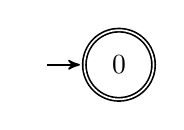
\begin{tikzpicture}[->,>=stealth',shorten >=1pt,auto,node distance=2.9cm,
                    semithick]
  \tikzstyle{every state}=[fill=white,text=black]
  \tikzstyle{place}=[rectangle,draw=black,fill=white, minimum size=7mm]

  \node[initial,state,accepting] (0)                    {$0$};
  
\end{tikzpicture}
\end{figure}

L'expression $a$ quant à elle est reconnue par 


\begin{figure}[H]
\centering
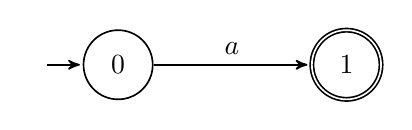
\begin{tikzpicture}[->,>=stealth',shorten >=1pt,auto,node distance=2.9cm,
                    semithick]
  \tikzstyle{every state}=[fill=white,text=black]
  \tikzstyle{place}=[rectangle,draw=black,fill=white, minimum size=7mm]


  \node[initial,state] (0)                    {$0$};
  \node[state,accepting] (1)      [right of=0]                {$1$};

  \path %(I) edge[loop above]              node {$a,b$} (I)
(0) edge      []        node {$a$} (1);

\end{tikzpicture}
\end{figure}

On peut donc traduire en automates les cas de base des expressions rationnelles. Quant aux cas récursifs, on les a en fait déjà traités en \ref{cloture} : pour construire un automate reconnaissant $e_1 + e_2$, on construit des automates $A_1$ et $A_2$ reconnaissant $e_1$ et $e_2$, et on applique la construction de l'union. On procède de même avec la concaténation pour $e_1e_2$ et l'itération pour $e^*$.
\end{proof}

%\paragraph*{Remarque} Les constructions vues pour les propriétés de clôture ne sont pas optimales. L'\href{https://fr.wikipedia.org/wiki/Algorithme_de_Thompson}{algorithme de Thomson} utilise les mêmes idées mais utilise les $\epsilon-transitions$ pour qu'il n'y ait pas plus d'un état initial et un état terminal tout au long de la construction de l'automate, ce qui permet de borner plus finement sa taille.

\subsection{Traduction linéaire}

On propose un autre algorithme, qui sépare la construction des états de celles des transitions : l'\textbf{algorithme de Glushkov}.

\begin{example}

Soit $e = (abb^*a+(ba)^*)^*$. On commence par distinguer toutes les lettres de l'expression, par exemple en les indexant par leur position. On obtient donc

\[
(a_1b_2b_3^*a_4+(b_5a_6)^*)^*
\]

On crée ensuite un état pour chaque lettre, ainsi qu'un état initial $0$ :


\begin{figure}[H]
\centering
\begin{tikzpicture}[->,>=stealth',shorten >=1pt,auto,node distance=2.5cm,
                    semithick]
  \tikzstyle{every state}=[fill=white,text=black]
  \tikzstyle{place}=[rectangle,draw=black,fill=white, minimum size=7mm]

  \node[initial,state] (0)                    {$0$};
  \node[state] (1)   [above right of=0]                {$a_1$};
  \node[state] (2)    [right of=1]     {$b_2$};
  \node[state] (3)             [right of=2]       {$b_3$};
  \node[state] (4)        [right of=3]            {$a_4$};
  \node[state] (5)     [below right of=0]               {$b_5$};
  \node[state] (6)     [right of=5]               {$a_6$};


%  \path %(I) edge[loop above]              node {$a,b$} (I)
%(0) edge      []        node {$a$} (1);

\end{tikzpicture}
\end{figure}

Le jeu va être de représenter, avec les transitions, les "promenades" dans l'expression. Toute mot capturé par l'expression commence par $a_1$ ou $b_5$. On ajoute donc ces transitions : 


\begin{figure}[H]
\centering
\begin{tikzpicture}[->,>=stealth',shorten >=1pt,auto,node distance=2.5cm,
                    semithick]
  \tikzstyle{every state}=[fill=white,text=black]
  \tikzstyle{place}=[rectangle,draw=black,fill=white, minimum size=7mm]

  \node[initial,state] (0)                    {$0$};
  \node[state] (1)   [above right of=0]                {$a_1$};
  \node[state] (2)    [right of=1]     {$b_2$};
  \node[state] (3)             [right of=2]       {$b_3$};
  \node[state] (4)        [right of=3]            {$a_4$};
  \node[state] (5)     [below right of=0]               {$b_5$};
  \node[state] (6)     [right of=5]               {$a_6$};


  \path %(I) edge[loop above]              node {$a,b$} (I)
(0) edge      []        node {$a_1$} (1)
(0) edge      []        node {$b_5$} (5)
;

\end{tikzpicture}
\end{figure}


Quand on a lu un $a_1$, on est obligé de lire un $b_2$. De même, un $b_5$ est forcément suivi d'un $a_6$ :

\begin{figure}[H]
\centering
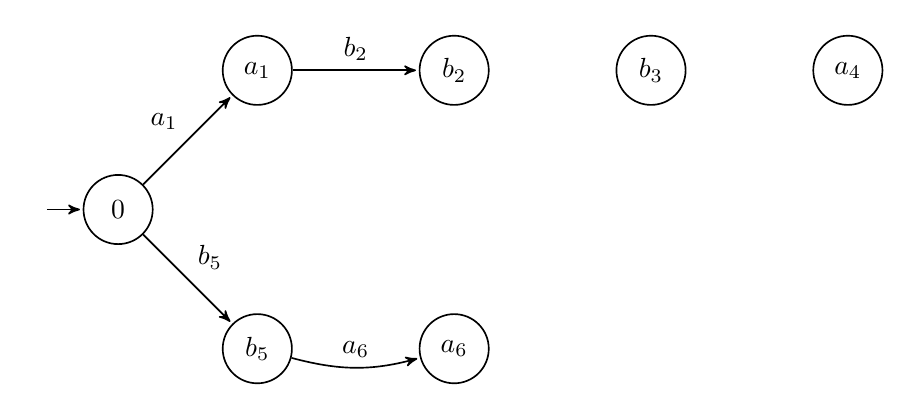
\begin{tikzpicture}[->,>=stealth',shorten >=1pt,auto,node distance=2.5cm,
                    semithick]
  \tikzstyle{every state}=[fill=white,text=black]
  \tikzstyle{place}=[rectangle,draw=black,fill=white, minimum size=7mm]

  \node[initial,state] (0)                    {$0$};
  \node[state] (1)   [above right of=0]                {$a_1$};
  \node[state] (2)    [right of=1]     {$b_2$};
  \node[state] (3)             [right of=2]       {$b_3$};
  \node[state] (4)        [right of=3]            {$a_4$};
  \node[state] (5)     [below right of=0]               {$b_5$};
  \node[state] (6)     [right of=5]               {$a_6$};


  \path %(I) edge[loop above]              node {$a,b$} (I)
(0) edge      []        node {$a_1$} (1)
(0) edge      []        node {$b_5$} (5)
(1) edge      []        node {$b_2$} (2)
(5) edge      [bend right=15]        node {$a_6$} (6)
;

\end{tikzpicture}
\end{figure}

Après la lecture d'un $a_6$, on peut recommencer la boucle $(b_5a_6)^*$, auquel cas on lit un $b_5$, ou recommencer la boucle entière $(a_1b_2b_3^*a_4+(b_5a_6)^*)^*$, en lisant un $a_1$ ou un $b_5$ :


\begin{figure}[H]
\centering
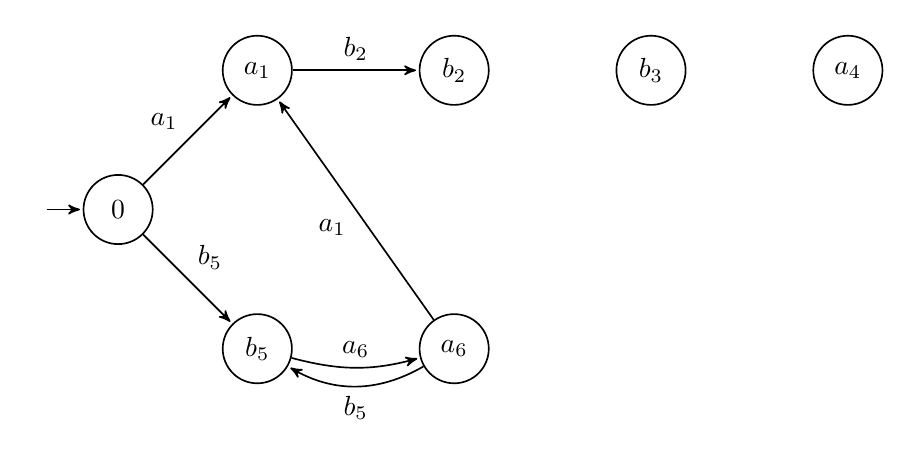
\begin{tikzpicture}[->,>=stealth',shorten >=1pt,auto,node distance=2.5cm,
                    semithick]
  \tikzstyle{every state}=[fill=white,text=black]
  \tikzstyle{place}=[rectangle,draw=black,fill=white, minimum size=7mm]

  \node[initial,state] (0)                    {$0$};
  \node[state] (1)   [above right of=0]                {$a_1$};
  \node[state] (2)    [right of=1]     {$b_2$};
  \node[state] (3)             [right of=2]       {$b_3$};
  \node[state] (4)        [right of=3]            {$a_4$};
  \node[state] (5)     [below right of=0]               {$b_5$};
  \node[state] (6)     [right of=5]               {$a_6$};


  \path %(I) edge[loop above]              node {$a,b$} (I)
(0) edge      []        node {$a_1$} (1)
(0) edge      []        node {$b_5$} (5)
(1) edge      []        node {$b_2$} (2)
(5) edge      [bend right=15]        node {$a_6$} (6)
(6) edge      [bend left]        node {$b_5$} (5)
(6) edge      []        node {$a_1$} (1)
;

\end{tikzpicture}
\end{figure}

Après la lecture d'un $b_2$, on peut lire un $b_3$, mais aussi sauter $b_3^*$ et aller directement lire un $a_4$. En $b_3$, on peut boucler ou passer en $a_4$. En $a_4$, comme en $a_6$, on peut lire $a_1$ ou $b_5$. On a donc :

\begin{figure}[H]
\centering
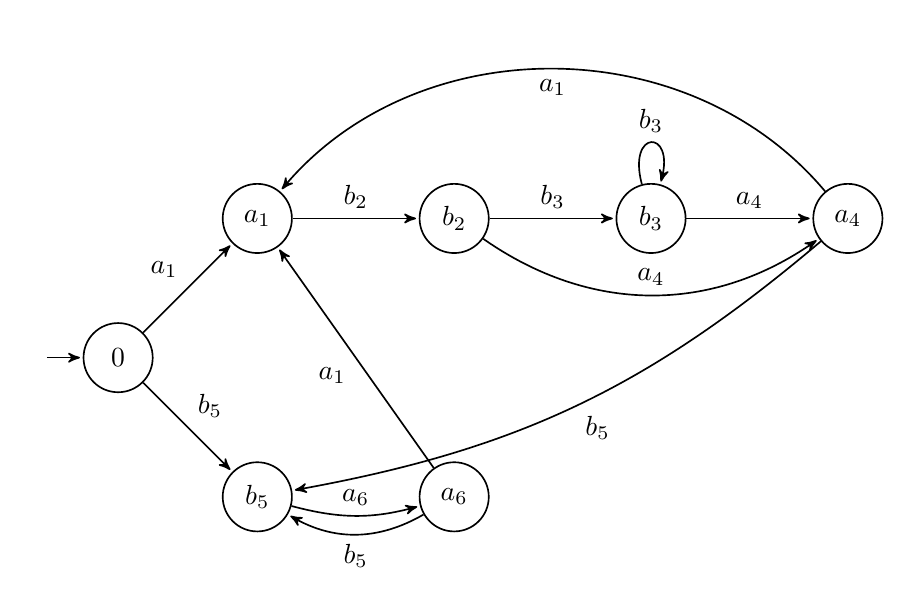
\begin{tikzpicture}[->,>=stealth',shorten >=1pt,auto,node distance=2.5cm,
                    semithick]
  \tikzstyle{every state}=[fill=white,text=black]
  \tikzstyle{place}=[rectangle,draw=black,fill=white, minimum size=7mm]

  \node[initial,state] (0)                    {$0$};
  \node[state] (1)   [above right of=0]                {$a_1$};
  \node[state] (2)    [right of=1]     {$b_2$};
  \node[state] (3)             [right of=2]       {$b_3$};
  \node[state] (4)        [right of=3]            {$a_4$};
  \node[state] (5)     [below right of=0]               {$b_5$};
  \node[state] (6)     [right of=5]               {$a_6$};


  \path %(I) edge[loop above]              node {$a,b$} (I)
(0) edge      []        node {$a_1$} (1)
(0) edge      []        node {$b_5$} (5)
(1) edge      []        node {$b_2$} (2)
(2) edge      []        node {$b_3$} (3)
(2) edge      [bend right=35]        node {$a_4$} (4)
(3) edge      []        node {$a_4$} (4)
(3) edge      [loop above]        node {$b_3$} (3)
(4) edge      [bend right=50]        node {$a_1$} (1)
(4) edge      [bend left=15]        node {$b_5$} (5)
(5) edge      [bend right=15]        node {$a_6$} (6)
(6) edge      [bend left]        node {$b_5$} (5)
(6) edge      []        node {$a_1$} (1)
;

\end{tikzpicture}
\end{figure}

On peut arrêter de boucler quand on vient de lire un $a_4$ ou un $a_6$, ce qui veut dire que les états correspondant vont être terminaux. De plus, l'expression rationnelle contient le mot vide, ce qui veut dire que l'état initial doit être terminal. Il ne nous reste plus qu'à "déspécialiser" les lettres, et éventuellement renommer les états :


\begin{figure}[H]
\centering
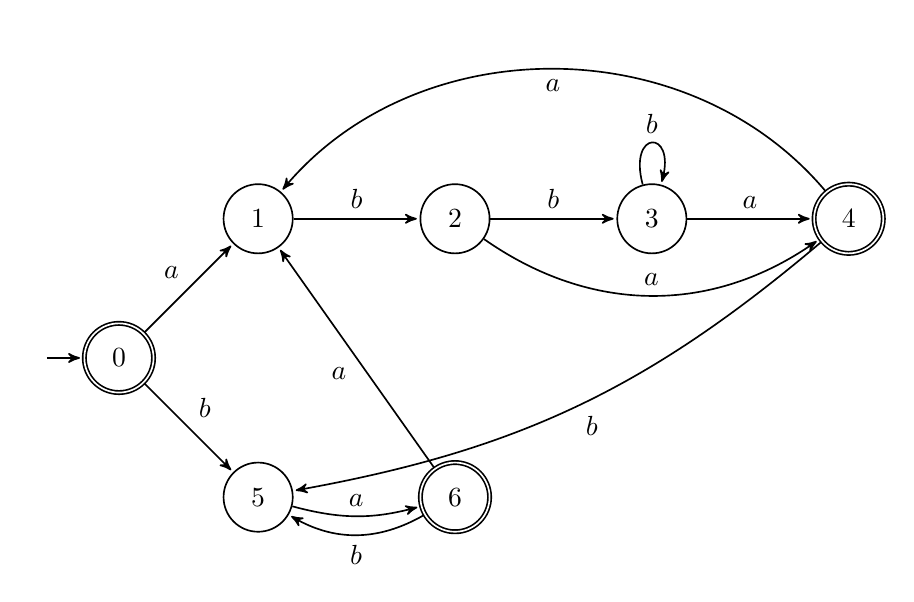
\begin{tikzpicture}[->,>=stealth',shorten >=1pt,auto,node distance=2.5cm,
                    semithick]
  \tikzstyle{every state}=[fill=white,text=black]
  \tikzstyle{place}=[rectangle,draw=black,fill=white, minimum size=7mm]

  \node[initial,state,accepting] (0)                    {$0$};
  \node[state] (1)   [above right of=0]                {$1$};
  \node[state] (2)    [right of=1]     {$2$};
  \node[state] (3)             [right of=2]       {$3$};
  \node[state,accepting] (4)        [right of=3]            {$4$};
  \node[state] (5)     [below right of=0]               {$5$};
  \node[state,accepting] (6)     [right of=5]               {$6$};


  \path %(I) edge[loop above]              node {$a,b$} (I)
(0) edge      []        node {$a$} (1)
(0) edge      []        node {$b$} (5)
(1) edge      []        node {$b$} (2)
(2) edge      []        node {$b$} (3)
(2) edge      [bend right=35]        node {$a$} (4)
(3) edge      []        node {$a$} (4)
(3) edge      [loop above]        node {$b$} (3)
(4) edge      [bend right=50]        node {$a$} (1)
(4) edge      [bend left=15]        node {$b$} (5)
(5) edge      [bend right=15]        node {$a$} (6)
(6) edge      [bend left]        node {$b$} (5)
(6) edge      []        node {$a$} (1)
;

\end{tikzpicture}
\end{figure}
\end{example}

On a présenté l'algorithme \textit{via} un exemple, mais il repose bien évidemment sur des définitions formelles, procédant par induction sur l'expression. Une fois qu'on a spécialisé les lettres et crée les états comme dans l'exemple, on veut d'abord savoir si l'expression rationnelle donnée accepte ou non le mot vide. C'est à cette question que répond la fonction suivante :

\[
\begin{cases}
E(\epsilon) = \top \\
E(a) = \bot \\
E(e_1+e_2) = E(e_1) \vee E(e_2) \\
E(e_1.e_2) = E(e_1) \wedge E(e_2) \\
E(e^*) = \top
\end{cases}
\]

L'état initial est $\top$ ssi. $E(e) = \top$. Pour les premières transitions, qui partiront de l'état initial $0$, on a besoin de déterminer quelles lettres peuvent commencer les mots reconnus par l'expression, ce que fait la fonction suivante : 

\[
\begin{cases}
D(\epsilon) = \emptyset \\
D(a) = \{a\} \\
D(e_1+e_2) = D(e_1) \cup D(e_2) \\
D(e_1.e_2) = D(e_1) & \text{Si } e_1 \text{ n'accepte pas le mot vide, cad. si }\neg E(e_1)\\
D(e_1.e_2) = D(e_1) \cup D(e_2) & \text{sinon}  \\
D(e^*) = D(e)
\end{cases}
\]

On ajoute une transition $0 \xrightarrow{q} q$ pour tout $q \in D(e)$. De même, on a besoin de savoir quelles lettres peuvent finir les mots du langage dénoté par une expression : 

\[
\begin{cases}
F(\epsilon) = \emptyset \\
F(a) = \{a\} \\
F(e_1+e_2) = F(e_1) \cup F(e_2) \\
F(e_1.e_2) = F(e_2) & \text{Si } e_2 \text{ n'accepte pas le mot vide, cad. si} \neg E(e_2)\\f
F(e_1.e_2) = F(e_1) \cup F(e_2) & \text{sinon}  \\
F(e^*) = F(e)
\end{cases}
\]


Tout les états de $F$ sont terminaux. En plus des premières transitions, on veut bien sûr les autres. Pour ça, on calcule l'ensemble des lettres qui peuvent se suivre dans le langage dénoté par l'expression :

\[
\begin{cases}
P(\epsilon) = \emptyset \\
P(a) = \emptyset \\
P(e_1+e_2) = P(e_1) \cup P(e_2) \\
P(e_1.e_2) = P(e_1) \cup P(e_2) \cup F(e_1).D(e_2) \\
P(e^*) = P(e) \cup F(e).D(e) 
\end{cases}
\]

Toute paire $\big \langle q_1, q_2 \big \rangle$ appartenant à $P(e)$ génère donc une transition $q_1 \xrightarrow{q_2} q_2$ dans l'automate.


\begin{exercice}
Utiliser l'algorithme de Glushkov pour traduire en automate l'expression \newline $e = (bb)^*(b(a+b)^*)^*$
\end{exercice}

\paragraph*{Remarque} On a présenté ces différents algorithmes comme des preuves de la "traductabilité" des expressions rationnelles en automates finis. Si on était vraiment rigoureux, les algorithmes ne suffiraient pas, il faudrait aussi prouver 1) qu'ils terminent sur toute entrée 2) qu'ils produisent bien un automate fini acceptant le langage décrit par l'expression donnée. Ces preuves sont autrement plus complexes que l'écriture des algorithmes\footnote{On entend souvent dire que la preuve d'un programme ou algorithme est au moins un ordre de grandeur plus complexe que l'écriture de ce dernier} et vont au-delà du programme du cours, mais il est toujours bon de garder son esprit critique face à ces choses. Cette remarque s'applique bien évidemment également à l'algorithme présenté dans les pages qui suivent pour la traduction inverse.


\bibliographystyle{plain}
\bibliography{poly}

\appendix


\chapter{Rappels mathématiques}
%\section{Lexique }

%\paragraph{}On rappelle quelques notions et notations de base.

\section{Logique}

\subsection{Raisonnement par l'absurde}
\label{abs}

\begin{definition}{Raisonnement par l'absurde}{}
Un \textbf{raisonnement par l'absurde} consiste à prouver une chose en 1) supposant son contraire et 2) montrer que ça fout tout en l'air. Plus formellement, pour prouver $P$, on suppose $\neg P$ et on montre que ça nous permet de déduire $\bot$, ce qui veut dire soit que la logique est incohérente, soit que $\neg P$ est fausse, et donc que $P$ est vraie.
\end{definition}

\begin{example}
Imaginons une situation où les rues sont sèches, et où on voudrait prouver qu'il n'a pas plu. On suppose alors l'inverse, c'est-à-dire qu'il a plu. Or, s'il a plu, les routes sont mouillées. On obtient alors que 1) les routes sont mouillées et 2) les routes ne sont pas mouillées, ce qui est un paradoxe. La seule hypothèse faite étant le fait qu'il a plu, elle doit être fausse.
\end{example}

\begin{example}
On veut prouver qu'il existe une infinité de nombres premiers. On suppose l'inverse, cad. qu'il y en a un ensemble fini $\{p_1,...,p_n\}$. Soit $n = 1 + \prod_{i \in [1 - n]} p_i = 1 + p_1 \times ... \times p_n$. $n$, comme tout nombre, admet au moins un diviseur premier. 

Or, $n$ est strictement plus grand que tout nombre premier et ne peut donc pas en être un. De plus, pour tout $i \in [1 - n]$, $\frac{n}{p_i} = p_1 \times ... \times p_{i-1} \times p_{i+1} \times ... \times p_n + \frac{1}{p_i}$. Tout nombre premier étant $\geq 2$, $\frac{1}{p_i}$ ne forme pas un entier, et donc $\frac{n}{p_i}$ non plus.

On obtient une contradiction, notre hypothèse sur la finitude des nombres premiers est donc fausse.
\end{example}



\section{Ensembles}

\subsection{Ensemble des parties}

Soit un ensemble $X$, on note $P(X)$ (parfois $2^X$) l'ensemble de ses parties, cad l'ensemble des ensembles formés à partir d'éléments de $X$.

\begin{example}
Soit $X = \{x,y,z\}$, alors - en classant les éléments par leur cardinal -

\begin{tabular}{llll}
 $P(X) = \{$ & $\emptyset$, & & \\
& $\{x\}$,&$\{y\}$,&$\{z\}$,\\
&$\{x,y\}$,& $\{x,z\}$,&$\{y,z\}$\\
& $\{x,y,z\}$ & &$~~~~~~~~\}$.
\end{tabular}
\end{example}

\begin{lemma}
$\forall X, \emptyset \in P(X) \wedge X \in P(X)$.
\end{lemma}

\begin{lemma}
$\forall X, |P(X)| = 2^{|X|}$.
\end{lemma}

\begin{proof}
Pour générer l'ensemble des sous-ensembles de $X$, on choisit de prendre ou non chaque élément de $X$. On a donc $\underbrace{2 \times 2 \times ... \times 2}_{\textrm{n fois}}$ choix, d'où les $2^{|X|}$ au total.
\end{proof}

\subsection{Opérations entre ensembles}

\begin{definition}{Produit d'ensembles}{}
\label{ensprod}
Soit deux ensembles $E_1$ et $E_2$, contenant respectivement des éléments de types $\tau_1$ et $\tau_2$. Soit également $\cdot$ une opération de type $\tau_1 \rightarrow \tau_2 \rightarrow \tau_3$, cad. une opération qui prend en argument gauche un élément de type $\tau_1$ et à droite un argument de type $\tau_2$ et renvoie un objet de type $\tau_3$, alors 

\[
E_1 \cdot E_2 = \{x \cdot y~|~x \in E_1~\wedge~y \in E_2\}
\]
\end{definition}

Dit autrement, un produit d'ensembles renvoie l'ensemble des combinaisons d'éléments de deux ensembles \textit{via} une opération fournie. Si l'opération $\cdot$ est un endormorphisme, cad. qu'elle est de type $\tau \rightarrow \tau \rightarrow \tau$, alors on peut itérer le produit de la façon suivante :

\begin{eqnarray*}
E^0 = \{1\} ~~~~~~~~~~~~~~~~ \textrm{Où $1$ est l'élément neutre de $\tau$} \\
E^{n+1} = E^n \cdot E
\end{eqnarray*}

Cette notion très générale ne doit pas être confondue avec

\begin{definition}{Produit cartésien}{}
Soit deux ensembles $E_1$ et $E_2$, ne contenant pas forcément des éléments de même type, alors

\[
E_1 \times E_2 = \{(x,y)~|~x \in E_1~\wedge~y \in E_2\}
\]
\end{definition}

Le produit cartésien, noté $\times$, renvoie l'ensemble des couples d'éléments de deux ensembles donnés. Il s'agit d'un cas particulier du produit d'ensemble, où l'opération est la "mise en couple". Cette opération ne pouvant pas être un endormorphisme, le produit cartésien ne peut être itéré.




\end{document}
